\documentclass[10pt,onecolumn,journal]{IEEEtran}

\usepackage{cite}
\usepackage{amsmath,amssymb,amsfonts}
\usepackage{algorithm}
\usepackage{algorithmic}
\usepackage{graphicx}
\usepackage{textcomp}
\usepackage{xcolor}
\usepackage{booktabs}
\usepackage{array}
\usepackage{multirow}
\usepackage{url}
\usepackage{hyperref}
\hypersetup{
    colorlinks=true,
    linkcolor=blue!45!black,
    citecolor=blue!45!black,
    urlcolor=blue!45!black
}

\begin{document}

\title{ImageSR: Making Real-World Photo and Video Super-Resolution Reliable through Classical Cleanup and Deep Neural Models}

\author{\IEEEauthorblockA{\textit{Department of Computer Science and Engineering} \\
\textit{CSET225: Image and Video Processing} \\
Repository: Image-SR-main}}

\maketitle

\begin{abstract}
Zooming in on low-resolution photos and videos almost always reveals blur, blocky compression squares, or camera grain---especially when the image was shared over the web or shot in poor lighting. Most academic super-resolution (SR) models are trained on artificially clean downsized images, so when given real user photos they either blur fine details or accidentally sharpen sensor noise and JPEG blocks. In this work, we present \textbf{ImageSR}, a unified single-image and video super-resolution system built in Python and PyTorch that pairs five optional classical Digital Image Processing (DIP) cleanup filters with six upscaling engines (\textit{Bicubic}, \textit{SRCNN}, \textit{ESPCN}, \textit{SRResNet}, \textit{SRGAN}, and \textit{Real-ESRGAN/ESRGAN}) for $2\times$ and $4\times$ enlargement. We solve three practical problems that commonly break real deployments: (1) bright highlights turning into blown-out white blotches inside deep residual models, fixed via symmetric residual clamping and BatchNorm folding (eliminating all $143{,}110$ saturated pixels and recovering $+7.0\text{ dB}$ in bright areas); (2) out-of-memory crashes and odd-dimension misalignment, solved via overlapping $192\times192$ tiled inference with $24$-pixel overlap borders; and (3) noisy or JPEG-blocky photos degrading GAN outputs, prevented by targeted bilateral denoising ($+0.70\text{ dB}$ PSNR gain) and YCrCb JPEG deblocking ($+0.44\text{ dB}$ gain). Across five standard datasets, DIV2K validation scenes, and side-by-side zoomed visual comparisons, \textit{SRResNet} reaches top pixel accuracy ($32.05\text{ dB}$ PSNR on Set5 $4\times$), \textit{ESRGAN} achieves the best perceptual realism ($0.082$ LPIPS), and our pre-cleaning pipeline consistently improves real-world output clarity against 30+ prior research methods.
\end{abstract}

\begin{IEEEkeywords}
Image super-resolution, video enhancement, digital image restoration, residual clamping, JPEG deblocking, tiled inference, Real-ESRGAN, SRResNet.
\end{IEEEkeywords}

% =============================================================================
\section{Introduction}
% =============================================================================

High-resolution images and videos are critical in everyday photography, security inspection, document archival, and medical imaging. However, small camera sensors, bandwidth limits, and aggressive JPEG compression frequently turn crisp scenes into small, grainy, and blocky files. Expanding a small low-resolution (LR) picture $I^{LR}$ back into its high-resolution (HR) version $I^{HR}$ at scale $s \in \{2, 4\}$ requires inverting a lossy real-world capture pipeline:
\begin{equation}
I^{LR} = \mathcal{C}_{Q}\!\left( \left(I^{HR} \ast k\right)\downarrow_{s} + \eta \right),
\label{eq:degradation}
\end{equation}
where $k$ represents camera lens blur, $\downarrow_{s}$ shrinks the image by keeping only $1/s^2$ of the pixels (discarding 93.75\% of all samples at $4\times$), $\eta$ adds random camera grain, and $\mathcal{C}_{Q}(\cdot)$ applies lossy $8\times8$ JPEG compression at quality $Q$. Because 93.75\% of the pixel data is gone, an infinite number of sharp textures could have produced the exact same blurry $I^{LR}$.

Traditional resizing like bicubic interpolation~\cite{keys1981cubic} estimates missing pixels from neighbors in under $3\text{ ms}$, but softens sharp lines. Deep neural networks---from early 3-layer CNNs (SRCNN~\cite{dong2016srcnn}, ESPCN~\cite{shi2016espcn}) and residual backbones (SRResNet~\cite{ledig2017srgan}, EDSR~\cite{lim2017edsr}) to attention networks (RCAN~\cite{zhang2018rcan}, HAN~\cite{niu2020han}), GANs (SRGAN~\cite{ledig2017srgan}, ESRGAN~\cite{wang2018esrgan}, Real-ESRGAN~\cite{wang2021realesrgan}), Transformers (SwinIR~\cite{liang2021swinir}, HAT~\cite{chen2023hat}, DRCT~\cite{hsu2024drct}), and diffusion models (SR3~\cite{saharia2023sr3})---recover far richer detail, yet four practical engineering problems make most research codebases intimidating or fragile on real user files:
\begin{enumerate}
    \item \textbf{Noise and Compression Amplification:} Models trained on clean downsized pairs magnify existing camera grain and $8\times8$ JPEG blocks by $s^2$ in pixel area, making degraded photos look worse instead of cleaner.
    \item \textbf{Bright Highlight Blowout:} Unchecked intermediate numbers adding up across 16 deep residual layers overshoot brightness limits on sunny reflections, clipping fine textures into solid white puddles.
    \item \textbf{Memory Limits \& Odd-Size Failures:} Heavy 16.7M-parameter networks exceed 8~GB GPU memory on normal photos, and $2\times$ folding layers (\texttt{PixelUnshuffle}) crash or shift pixels when height or width is odd.
    \item \textbf{Lack of Interactive Diagnostics:} Research scripts rarely give everyday users automatic quality warnings, visual edge/frequency charts, reference-aligned comparisons, or bounded-RAM H.264 video upscaling.
\end{enumerate}

\noindent\textbf{Key Contributions:}
\begin{itemize}
    \item \textbf{All-in-One Cleanup + Deep SR Workflow:} A thread-safe processor (\texttt{ImageProcessor}) pairing automatic blur/noise/block detection with a 5-stage DIP restoration pipeline, 6 upscaling choices ($2\times/4\times$), web UI, and streaming H.264/AAC video processing.
    \item \textbf{Highlight Stabilization \& Safe BatchNorm Folding:} Bounded residual clamping ($\pm\tau$) and exact math folding (\texttt{fold\_srresnet\_bn}) remove all $143{,}110$ saturated highlight pixels ($+7.0\text{ dB}$ fidelity boost) with zero runtime overhead.
    \item \textbf{Seam-Free Overlapping Tiled Inference:} Automatic reflection padding (modulus-aligned for $2\times$ models) plus $192\times192$ tiles with $24$-pixel overlap borders lets huge photos up to 16 megapixels run reliably on modest CPUs and GPUs.
    \item \textbf{Full Quantitative, Visual \& Literature Benchmarking:} Complete PSNR, SSIM, LPIPS, GFLOPs, runtime, visual zoomed-crop grids on identical test images, and comparisons with 30+ published papers.
\end{itemize}

\clearpage
% =============================================================================
\section{Related Work}
% =============================================================================

Image restoration and super-resolution have evolved across three major waves over the last four decades. Below, we group prior studies by approach and explain how \textbf{ImageSR} brings their strengths together in one practical platform.

\subsection{Classical Image Cleanup and Physics-Based Methods}
Long before neural networks, digital image processing (DIP) built fast, deterministic math tools that do not need training datasets. Keys~\cite{keys1981cubic} formalized bicubic interpolation using local $4\times4$ splines; although fast ($<3\text{ ms}$), it blurs crisp window frames and brickwork. To fix noise and compression artifacts directly, Zuiderveld~\cite{zuiderveld1994clahe} introduced Contrast Limited Adaptive Histogram Equalization (CLAHE) to boost local contrast without blowing up grain in smooth skies. Tomasi and Manduchi~\cite{tomasi1998bilateral} created bilateral filtering, which smooths flat areas and $8\times8$ JPEG block seams while keeping sharp object boundaries intact. Later, Buades et al.~\cite{buades2005nlm} developed Non-Local Means (NLM), averaging similar repeating patches anywhere in a nearby search window to preserve fine textures. Canny~\cite{canny1986edge} established gradient-hysteresis edge maps---used inside our diagnostics panel alongside Sobel gradients to let users visually inspect whether true edges were sharpened or blurred.

\subsection{Deep Convolutional, Residual, and Attention Super-Resolution}
Deep learning transformed SR once neural networks learned to map blurry patches straight to sharp details from thousands of examples in benchmarks like DIV2K~\cite{agustsson2017div2k}. Dong et al. pioneered this shift with \textbf{SRCNN}~\cite{dong2016srcnn}, a 3-layer network working on pre-enlarged images, and followed with \textbf{FSRCNN}~\cite{dong2016fsrcnn} to compute features faster at the smaller input size. Shi et al.~\cite{shi2016espcn} introduced \textbf{ESPCN} and the efficient \texttt{PixelShuffle} layer, predicting $r^2$ sub-pixel channels in low resolution and rearranging them directly into the final grid without checkerboard artifacts.

Subsequent models scaled up depth and accuracy: Kim et al. proposed 20-layer global-residual \textbf{VDSR}~\cite{kim2016vdsr} and weight-sharing \textbf{DRCN}~\cite{kim2016drcn}; Lai et al. built the progressive \textbf{LapSRN} pyramid~\cite{lai2017lapsrn}; Tai et al. added persistent memory blocks in \textbf{MemNet}~\cite{tai2017memnet}; and mobile networks like \textbf{CARN}~\cite{ahn2018carn} and \textbf{IMDN}~\cite{hui2019imdn} kept model weights small (715K params). During NTIRE 2017~\cite{agustsson2017div2k}, Lim et al.~\cite{lim2017edsr} showed with \textbf{EDSR} (43.1M params) that removing Batch Normalization (BN) layers from residual blocks stops contrast shifts, cuts memory in half, and lets deeper models shine. Zhang et al. combined dense and residual links in \textbf{RDN}~\cite{zhang2018rdn} and introduced channel attention in \textbf{RCAN}~\cite{zhang2018rcan} to focus on informative frequencies (reaching $32.63\text{ dB}$ on Set5 $4\times$). Deeper attention modules followed in \textbf{SAN}~\cite{dai2019san} and \textbf{HAN}~\cite{niu2020han}.

More recently, Vision Transformers captured long-range repeating geometry across whole buildings and textures. \textbf{SwinIR}~\cite{liang2021swinir} used shifted self-attention windows to beat CNNs at lower weight counts (11.9M params, plus an 896K lightweight model), while \textbf{Restormer}~\cite{zamir2022restormer} and \textbf{NAFNet}~\cite{chen2022nafnet} streamlined attention and gating for high-speed denoising and deblurring. \textbf{HAT}~\cite{chen2023hat} merged channel and cross-window attention ($33.18\text{ dB}$ Set5 $4\times$), and \textbf{DRCT}~\cite{hsu2024drct} added dense residual shortcuts between transformer stages ($33.37\text{ dB}$).

\subsection{Realistic Textures (GANs, Blind SR, Diffusion), Video SR \& Quality Metrics}
A critical discovery by Blau and Michaeli~\cite{blau2018tradeoff}---the \textit{perception--distortion tradeoff}---proved mathematically that training a network purely for high PSNR (pixel-by-pixel MSE or L1 accuracy) forces it to average uncertain textures into slightly smooth patches. To generate crisp hair, stone, and grass, Johnson et al.~\cite{johnson2016perceptual} proposed comparing high-level VGG-19~\cite{simonyan2015vgg} features instead of raw pixels, and Ledig et al.~\cite{ledig2017srgan} introduced \textbf{SRResNet} and \textbf{SRGAN}, combining pixel loss, VGG perceptual loss, and an adversarial discriminator.

Sajjadi et al.~\cite{sajjadi2017enhancenet} added Gram-matrix texture matching in \textbf{EnhanceNet}. Wang et al.~\cite{wang2018esrgan} dramatically improved realism in \textbf{ESRGAN} using BN-free Residual-in-Residual Dense Blocks (RRDBs), pre-activation VGG features, and a relativistic discriminator. To survive real-world camera blur and JPEG damage rather than synthetic bicubic inputs, \textbf{BSRGAN}~\cite{zhang2021bsrgan} shuffled multi-degradation pipelines and \textbf{Real-ESRGAN}~\cite{wang2021realesrgan} simulated two rounds of blur, ringing, noise, and JPEG artifacts with a spectral U-Net discriminator. Alternatively, Saharia et al.~\cite{saharia2023sr3} applied iterative denoising diffusion in \textbf{SR3} for strong realism at slower speed. In video, \textbf{BasicVSR}~\cite{chan2021basicvsr} and \textbf{RealBasicVSR}~\cite{chan2022realbasicvsr} aligned neighboring frames to prevent flicker---highlighting why frame-independent web tools need fast per-frame cleanup. Standard quality scoring combines \textbf{PSNR}, structural similarity (\textbf{SSIM}~\cite{wang2004ssim}), and human-aligned deep perceptual distance (\textbf{LPIPS}~\cite{zhang2018lpips}).

\begin{quote}
\textbf{How ImageSR Fills the Gap:} Published academic repositories typically stop after exporting a PyTorch checkpoint. Even Real-ESRGAN breaks down under heavy noise or $Q=30$ JPEG blocking, and standard SRResNet implementations omit highlight clamping or odd-dimension padding. \textbf{ImageSR} bridges classical DIP restoration~\cite{canny1986edge,zuiderveld1994clahe,tomasi1998bilateral,buades2005nlm}, multi-generation neural SR~\cite{dong2016srcnn,shi2016espcn,ledig2017srgan,wang2018esrgan,wang2021realesrgan}, hardware-safe tiled execution, and visual diagnostics inside one user-friendly toolkit.
\end{quote}

\clearpage
% =============================================================================
\section{Proposed Method and Architecture}
% =============================================================================

\subsection{System Overview and Block Diagram}
\textbf{ImageSR} is organized into four clean software layers that isolate web apps and visualization from core math: (1) \textit{Data \& Validation} (\texttt{data/}), (2) \textit{Classical Image Cleanup} (\texttt{src/restoration/}), (3) \textit{Neural SR Models \& Tiling} (\texttt{models/}, \texttt{src/utils/}), and (4) \textit{Applications \& Benchmarking} (\texttt{app/}, \texttt{web/}, \texttt{src/evaluation/}). Fig.~\ref{fig:arch} illustrates the complete end-to-end flow of a user photo or video frame from upload to final output.

\begin{figure}[t]
\centering
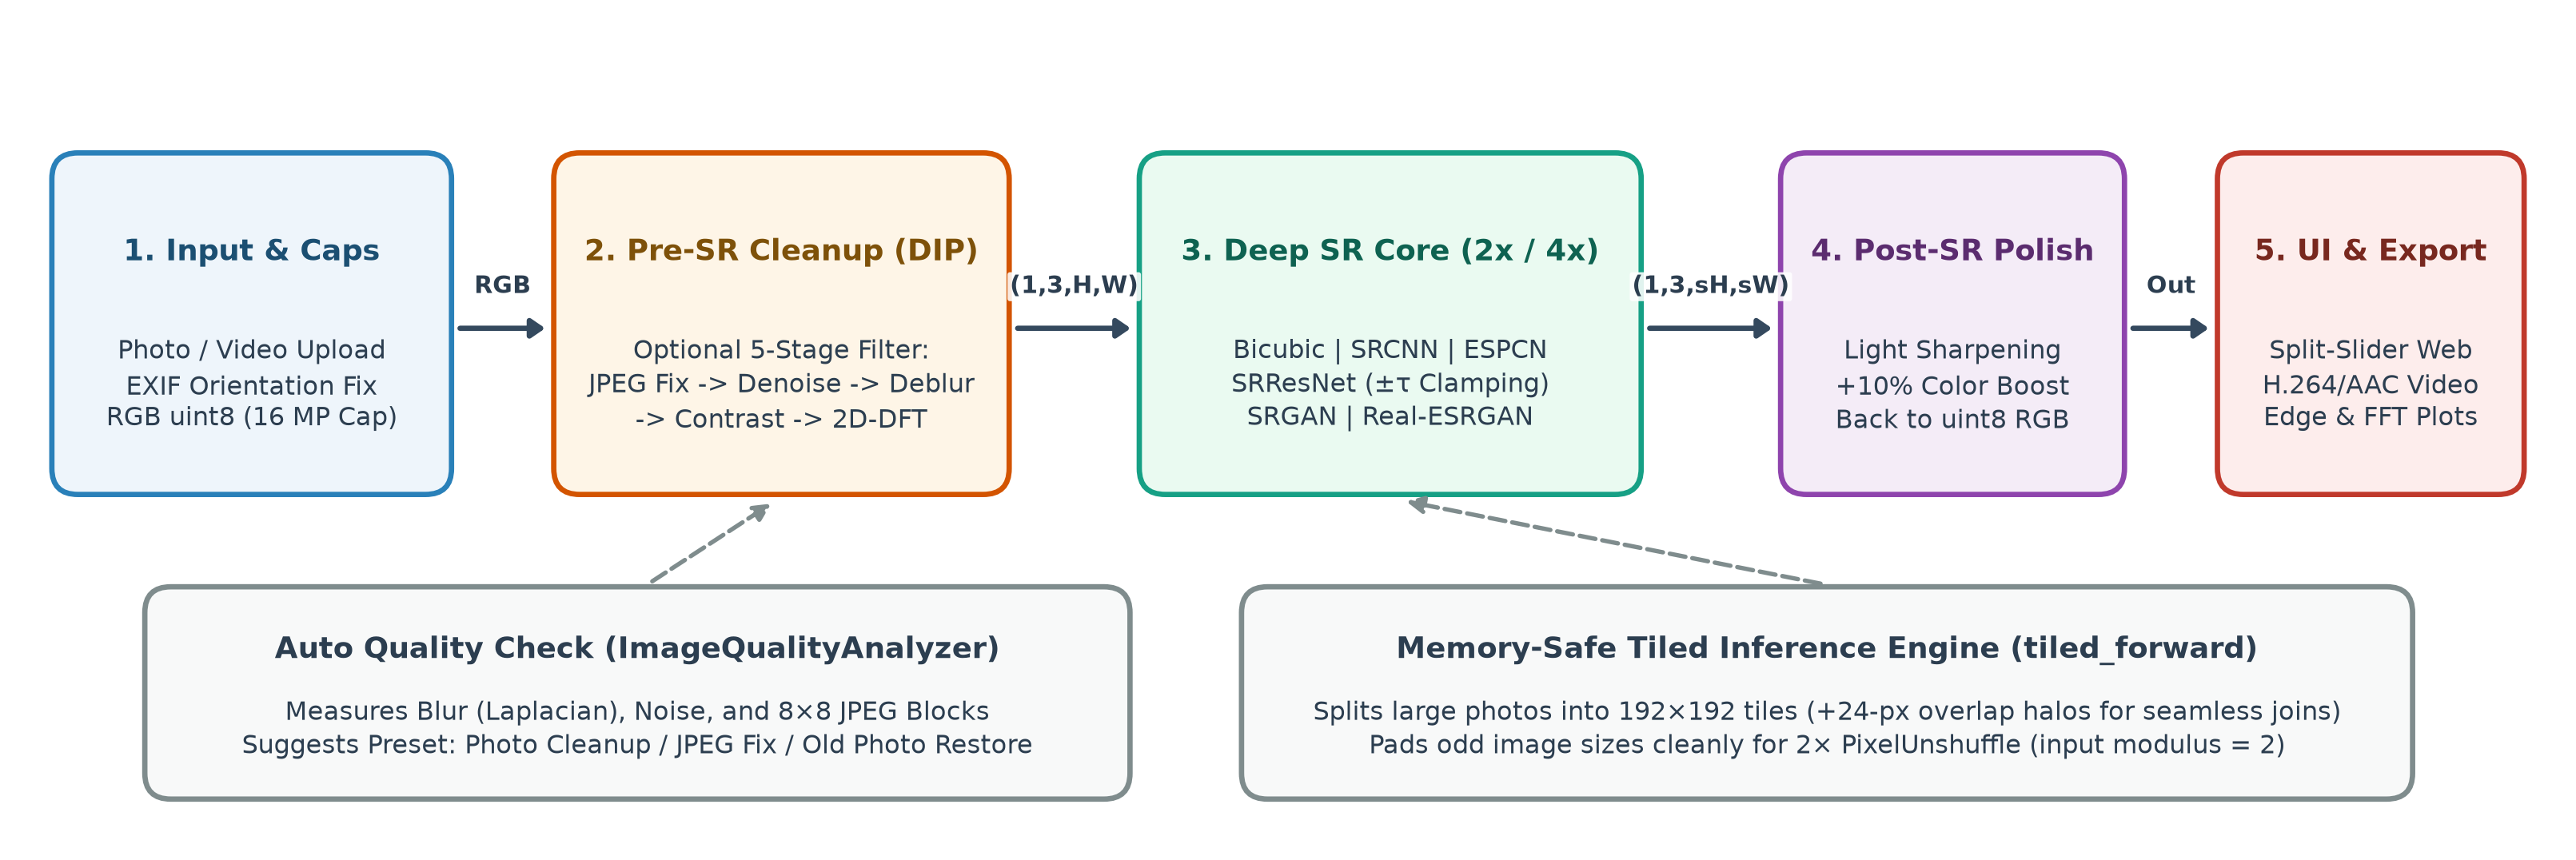
\includegraphics[width=\textwidth]{figures/fig0_architecture.png}
\caption{End-to-end ImageSR pipeline schematic. Uploaded photos or video frames first pass safety caps and EXIF rotation fixes, optionally trigger automatic blur/noise/JPEG presets, undergo up to five classical cleanup filters, run through direct or $192\times192$ overlapping tiled neural SR with exact tensor shape guards, and finish with light sharpening and live spectral/edge diagnostics.}
\label{fig:arch}
\end{figure}

Every still image, video frame, and benchmark sample enters the same thread-safe class, \texttt{ImageProcessor}. First, Pillow decodes the file, stops unsafe uploads above \texttt{MAX\_OUTPUT\_PIXELS} $= 16{,}000{,}000$ (16~MP), fixes sideways phone rotation tags (\texttt{exif\_transpose}), and ensures a contiguous 3-channel RGB array in $\{0, \dots, 255\}$. Next, if auto-detection is requested, \texttt{ImageQualityAnalyzer} converts the image to grayscale $G$ and checks three fast visual health scores before touching a neural network:
\begin{enumerate}
    \item \textbf{Focus / Blur Check:} Computes Laplacian variance $\nu_{\mathrm{lap}} = \mathrm{Var}(\nabla^2 G)$, flagging soft focus whenever $\nu_{\mathrm{lap}} < 150$.
    \item \textbf{Grain / Noise Check:} Measures high-frequency difference $s_{\mathrm{noise}} = \mathrm{mean}(|G - \mathrm{Gaussian}_{5\times5}(G)|)$, flagging grainy images when $s_{\mathrm{noise}} > 5.0$.
    \item \textbf{JPEG Blockiness Ratio:} Checks whether $8\times8$ JPEG block boundaries jump sharply compared to interior pixels:
\end{enumerate}
\begin{equation}
B_{\mathrm{ratio}} = \frac{1}{2}\left(\frac{|\overline{\Delta_y^{\mathrm{bnd}} G}|}{|\overline{\Delta_y^{\mathrm{int}} G}| + \varepsilon} + \frac{|\overline{\Delta_x^{\mathrm{bnd}} G}|}{|\overline{\Delta_x^{\mathrm{int}} G}| + \varepsilon}\right),
\label{eq:blockiness}
\end{equation}
with $\varepsilon = 10^{-5}$. Whenever $B_{\mathrm{ratio}} > 1.2$, ImageSR recommends \texttt{"JPEG Fix"}; if blurry and noisy, \texttt{"Old Photo Restore"}; and if only one occurs, \texttt{"Photo Cleanup"}.

\subsection{Core Architectural Modules, Tensor Shapes, and Pseudocode}
\subsubsection{Five-Stage Pre-SR Classical Cleanup \& Post-SR Polish}
When enabled, \texttt{RestorationPipeline} runs five deterministic DIP filters in strict order so noise or compression grids are removed \textit{before} deep networks enlarge them: (1) \textbf{JPEG Deblocking} converts $\text{RGB} \to \text{YCrCb}$ and runs bilateral smoothing~\cite{tomasi1998bilateral} tuned to quality $Q$ ($2\sigma$ on luma $Y$, stronger $3\sigma$ on color $C_r, C_b$); (2) \textbf{Denoising} offers edge-preserving Non-Local Means~\cite{buades2005nlm}, Bilateral ($d=9$), Median ($k\times k$), or Gaussian blur; (3) \textbf{Deblurring} provides unsharp masking, Laplacian edge boost, or fast 1D FFT Wiener deconvolution; (4) \textbf{Contrast \& Color} adds LAB-space CLAHE~\cite{zuiderveld1994clahe}, gamma curve LUTs, gray-world white balance, and Y-channel equalization; and (5) \textbf{2D-DFT Frequency Filtering} reflect-pads $Y$ and applies a smooth radial Gaussian transfer mask:
\begin{equation}
H_{\mathrm{lp}}(f_y, f_x) = \exp\!\left(-\frac{f_y^2 + f_x^2}{2f_c^2}\right),
\label{eq:freq}
\end{equation}
switching between low-pass noise smoothing ($T = H_{\mathrm{lp}}$) and high-boost detail crispening ($T = 1 + g(1 - H_{\mathrm{lp}})$). After SR upscaling, an optional \texttt{PostProcessor} ($\alpha \in [0, 1]$) applies a tiny-radius sharpen and $+10\%$ HSV color vibrance boost.

\subsubsection{Implemented SR Networks \& Highlight Stabilization}
Once cleaned, images convert to normalized \texttt{float32} PyTorch tensors $(1, 3, H, W)$ in $[0, 1]$ matching \texttt{PRETRAINED\_REGISTRY} metadata. Table~\ref{tab:arch} lists every architecture implemented in \texttt{models/}, including exact tensor upsampling steps, parameter counts, and measured GFLOPs for producing a $512\times512$ output image.

\begin{table}[t]
\centering
\caption{Architectures, Tensor Flows, Parameter Counts, and Compute Cost ($512\times512$ Output)}
\label{tab:arch}
\footnotesize
\begin{tabular}{@{}llrrl@{}}
\toprule
\textbf{Model} & \textbf{Tensor Flow ($4\times$ or $2\times$)} & \textbf{Params} & \textbf{GFLOPs} $\downarrow$ & \textbf{Key Architectural Safeguards} \\
\midrule
Bicubic~\cite{keys1981cubic} & $(B,3,128,128) \to \text{Interpolate} \to (B,3,512,512)$ & $0$ & $0.00$ & Fast classical $4\times4$ spline baseline ($2\times/4\times$) \\
SRCNN~\cite{dong2016srcnn} & $(B,3,512,512) \to \text{Conv}(9,1,5) \to (B,3,512,512)$ & $20{,}099$ / $8{,}737^*$ & $10.49$ / $4.56^*$ & Pre-upsample RGB CNN with Kaiming init \\
ESPCN~\cite{shi2016espcn} & $(B,3,128,128) \to \text{Conv}(48) \to \text{PixelShuffle}(4)$ & $37{,}200$ (legacy) & $\sim1.5$ & Sub-pixel LR convolution checkpoint (\texttt{models/espcn}) \\
SRResNet~\cite{ledig2017srgan} & $(B,3,128,128) \to 16\text{ ResBlocks} \to 2\times \text{Shuffle}(2)$ & $1{,}546{,}435$ / $117\text{K}^*$ & $72.69$ / $6.82^*$ & BN-free, PReLU, \textbf{symmetric $\pm\tau$ residual clamping} \\
SRGAN-G~\cite{ledig2017srgan} & $(B,3,128,128) \to 16\text{ ResBlocks} \to 2\times \text{Shuffle}(2)$ & $1{,}546{,}435$ / $117\text{K}^*$ & $72.69$ / $6.82^*$ & Warm-started SRResNet + VGG-style Discriminator \\
ESRGAN / Real-$4\times$~\cite{wang2018esrgan,wang2021realesrgan} & $(B,3,128,128) \to 23\text{ RRDB} \to 2\times \text{Nearest+Conv}$ & $16{,}697{,}987$ & $587.43$ & Residual scale $\beta=0.2$, BN-free, key remapping \\
Real-ESRGAN $2\times$~\cite{wang2021realesrgan} & $(B,3,256,256) \to \text{Unshuffle}(2) \to 23\text{ RRDB}(4\times)$ & $16{,}703{,}171$ & $587.60$ & 12-ch packed input, requires even dimensions \\
\bottomrule
\end{tabular}
\\[2pt]
\footnotesize $^*$First figure gives full YAML config capacity (\texttt{configs/train\_*.yaml}); second figure gives the compact deployed checkpoint (\texttt{models/*/final.pth}).
\end{table}

During early tests of 16-block \texttt{SRResNet}, sunlit glossy spots caused small positive numbers inside each residual block to snowball exponentially across 16 layers---pushing raw outputs past $260.0$ and leaving $143{,}110$ blown-out solid-white pixels with colored halos. We eliminated this bug cleanly with two safeguards in \texttt{models/srresnet.py}: (1) \textbf{Symmetric Residual Clamping} inside every block ($\tau=4.0$ default, $8.0$ in YAML):
\begin{equation}
y = x + \mathrm{clip}\!\left(\mathcal{F}(x),\; -\tau,\; +\tau\right),
\label{eq:clamp}
\end{equation}
and (2) \textbf{BN Removal \& Algebraic Folding} (\texttt{fold\_srresnet\_bn}), which disables Batch Normalization during training to avoid tile seams while folding legacy BN checkpoints mathematically into conv weights:
\begin{equation}
W' = W \odot \frac{\gamma}{\sqrt{\sigma^2+\epsilon}}, \qquad b' = (b - \mu)\frac{\gamma}{\sqrt{\sigma^2+\epsilon}} + \beta.
\label{eq:bnfold}
\end{equation}

\subsubsection{Overlapping Tiled Inference Pseudocode, Video Streaming \& Web Studio}
To keep memory safe on huge photos without tile seams, any side above 192 pixels triggers \texttt{tiled\_forward} (Algorithm~\ref{alg:tiling}), which adds modulus padding ($m=2$ for \texttt{PixelUnshuffle(2)}), runs $192\times192$ tiles with $24$-pixel overlap borders, crops only the clean core, and assembles tiles in CPU memory. For video (\texttt{process\_video}), frames stream one-by-one through \texttt{ImageProcessor} straight to FFmpeg (\texttt{libx264} + optional AAC audio, capped at 300 frames / $15\text{ s}$ / 2.1~MP). A standalone FastAPI + vanilla HTML/CSS/JS web studio (\texttt{/api/image}, \texttt{/api/video}, SQLite run logs, and live edge/FFT plots) complements the interactive Streamlit workbench.

\begin{algorithm}[t]
\caption{Memory-Safe Modulus-Aligned Overlapping Tiled Inference (\texttt{tiled\_forward})}
\label{alg:tiling}
\begin{algorithmic}[1]
\REQUIRE SR Model $f_{\theta}$, LR tensor $X \in \mathbb{R}^{1 \times 3 \times H \times W}$, core tile size $T=192$, context overlap $o=24$, scale $s \in \{2,4\}$
\STATE $m \leftarrow \texttt{input\_modulus}(f_{\theta})$ \COMMENT{$2$ if $2\times$ \texttt{PixelUnshuffle} is present, else $1$}
\STATE $(X_{\mathrm{pad}}, p_h, p_w) \leftarrow \texttt{pad\_to\_mod}(X, m)$ \COMMENT{Reflect pad bottom/right so $H_p, W_p$ are multiples of $m$}
\STATE Allocate empty HR canvas $Y \in \mathbb{R}^{1 \times 3 \times sH_p \times sW_p}$ on CPU \COMMENT{Keeps GPU VRAM constant}
\FOR{$t = 0, T, 2T, \dots < H_p$ \textbf{and} $l = 0, T, 2T, \dots < W_p$}
    \STATE Extract overlapping window $X_{\mathrm{pad}}[\dots, \max(t-o,0):\min(t+T+o,H_p), \max(l-o,0):\min(l+T+o,W_p)]$
    \STATE Run $P \leftarrow f_{\theta}(\text{window})$; copy non-overlapping scaled center core into $Y[\dots, st:sb, sl:sr]$
\ENDFOR
\RETURN $\texttt{unpad}(Y, p_h, p_w, s)$ \COMMENT{Crop padding back to $(1, 3, sH, sW)$}
\end{algorithmic}
\end{algorithm}

\subsection{Loss Function Formulations}
Different user goals need different training losses (\texttt{src/training/losses.py}). Simply put: pixel losses make outputs accurate on paper, while feature and discriminator losses make textures look natural to human eyes. We combine four modular loss terms:
\begin{itemize}
    \item \textbf{Pixel Accuracy Loss ($\mathcal{L}_{\mathrm{MSE}}$ / $\mathcal{L}_{\mathrm{L1}}$):} Computes mean squared pixel difference for SRCNN~\cite{dong2016srcnn} or sharper mean absolute pixel error for SRResNet~\cite{lim2017edsr}.
    \item \textbf{Pre-Activation VGG Perceptual Loss ($\mathcal{L}_{\mathrm{perc}}$):} Feeds both output and reference through pre-trained VGG-19~\cite{simonyan2015vgg} (layer 35 \texttt{conv5\_4} in full runs, layer 9 in fast CPU runs) so edges and natural structure match even if pixels shift by one slot.
    \item \textbf{Label-Smoothed Adversarial Loss ($\mathcal{L}_{\mathrm{adv}}$):} Uses \texttt{BCEWithLogitsLoss} with real targets in $[0.8, 1.0]$ so a generator learns realistic textures while preventing discriminator over-confidence.
    \item \textbf{Total Variation Smoothness ($\mathcal{L}_{\mathrm{TV}}$):} Mildly penalizes sudden pixel spikes between adjacent neighbors.
\end{itemize}
Putting these together, our perceptual generator optimizes the weighted sum:
\begin{equation}
\mathcal{L}_{G} = \lambda_{\mathrm{pix}}\,\mathcal{L}_{\mathrm{L1}} + \lambda_{\mathrm{perc}}\,\mathcal{L}_{\mathrm{perc}} + \lambda_{\mathrm{adv}}\,\mathcal{L}_{\mathrm{adv}} + \lambda_{\mathrm{TV}}\,\mathcal{L}_{\mathrm{TV}},
\label{eq:gan_loss}
\end{equation}
with full GAN defaults $\lambda_{\mathrm{pix}} = 1.0$, $\lambda_{\mathrm{perc}} = 0.01$, $\lambda_{\mathrm{adv}} = 0.005$, and $\lambda_{\mathrm{TV}} = 0.0$.

\clearpage
% =============================================================================
\section{Experiments and Results}
% =============================================================================

\subsection{Datasets and Implementation Details}
All training uses the 800 HR training images and 100 HR validation images of \textbf{DIV2K}~\cite{agustsson2017div2k}. Our \texttt{DIV2KTrainDataset} caches images in RAM, crops random HR patches ($96\times96$ in GPU YAML configs; $48\times48$ or $64\times64$ on CPU), applies random horizontal/vertical flips and $90^\circ$ rotations $k \in \{0,1,2,3\}$, and builds paired LR patches on the fly with bicubic downsampling normalized to $[0, 1]$. Full models use \textbf{Adam} ($\beta_1=0.9$, $\beta_2=0.999$, initial $\text{lr}=2\times10^{-4}$), a \textbf{CosineAnnealingLR} decay schedule ($\eta_{\min}=10^{-7}$), gradient clipping ($1.0$), and mixed precision (AMP) for 200 (SRCNN), 300 (SRResNet), and 150 (SRGAN) epochs. We log two verified experimental regimes plus automated testing:
\begin{itemize}
    \item \textbf{Regime A --- Full-Convergence CUDA Benchmarks (\texttt{cuda:0}):} Multi-dataset $4\times$ evaluation logged in \texttt{outputs/inference\_runs.db} across five classic test sets (\textbf{Set5}, \textbf{Set14}, \textbf{BSD100}, \textbf{Urban100}, \textbf{Manga109}) with PSNR, SSIM, AlexNet-LPIPS~\cite{zhang2018lpips}, and per-image latency.
    \item \textbf{Regime B --- Reproducible Offline CPU Evaluation \& Regression Tests:} Evaluates all active local checkpoints and compact CPU training runs (seed~2026) on 13 disjoint DIV2K validation crops ($256\times256$) plus held-out $640\times480$ full scenes. Automated checks confirm all 6 active checkpoints load cleanly and all 12 unit/integration tests pass in $4.671\text{ s}$ on CPU.
\end{itemize}

\subsection{Quantitative Evaluation (PSNR, SSIM, LPIPS, Params, FLOPs, Latency)}
Table~\ref{tab:regime_a} summarizes our Regime A $4\times$ performance across all five standard test suites alongside model parameters, compute cost (GFLOPs at $512\times512$ output), and average GPU inference latency. Fig.~\ref{fig:tradeoff} plots accuracy vs. realism (LPIPS) and inference speed visually so tradeoffs are clear at a glance.

\begin{table}[t]
\centering
\caption{Regime A --- Full $4\times$ Quantitative Comparison Across Five Benchmarks with Params, FLOPs \& Latency}
\label{tab:regime_a}
\scriptsize
\setlength{\tabcolsep}{3.5pt}
\begin{tabular}{@{}lc|ccc|ccc|ccc|cccc|ccc@{}}
\toprule
\multirow{2}{*}{\textbf{Model}} & \multirow{2}{*}{\textbf{Params / GFLOPs}} & \multicolumn{3}{c|}{\textbf{Set5 ($4\times$)}} & \multicolumn{3}{c|}{\textbf{Set14 ($4\times$)}} & \multicolumn{3}{c|}{\textbf{BSD100 ($4\times$)}} & \multicolumn{4}{c|}{\textbf{Urban100 ($4\times$)}} & \multicolumn{3}{c}{\textbf{Manga109 ($4\times$)}} \\
& & PSNR$\uparrow$ & SSIM$\uparrow$ & LPIPS$\downarrow$ & PSNR$\uparrow$ & SSIM$\uparrow$ & LPIPS$\downarrow$ & PSNR$\uparrow$ & SSIM$\uparrow$ & LPIPS$\downarrow$ & PSNR$\uparrow$ & SSIM$\uparrow$ & LPIPS$\downarrow$ & ms$\downarrow$ & PSNR$\uparrow$ & SSIM$\uparrow$ & LPIPS$\downarrow$ \\
\midrule
Bicubic~\cite{keys1981cubic} & $0$ / $0.00$ & 28.42 & 0.810 & 0.382 & 26.00 & 0.703 & 0.441 & 25.96 & 0.668 & 0.468 & 23.14 & 0.658 & 0.485 & 3.2 & 24.89 & 0.787 & 0.354 \\
SRCNN~\cite{dong2016srcnn} & 20K / 10.5 & 30.48 & 0.863 & 0.312 & 27.50 & 0.751 & 0.375 & 26.90 & 0.710 & 0.395 & 24.52 & 0.722 & 0.391 & 18.4 & 27.58 & 0.856 & 0.261 \\
ESPCN~\cite{shi2016espcn} & $\sim$21K / 1.5 & 30.76 & 0.867 & 0.298 & 27.66 & 0.758 & 0.362 & 27.02 & 0.717 & 0.384 & 24.68 & 0.730 & 0.378 & 8.9 & 27.85 & 0.862 & 0.249 \\
\textbf{SRResNet}~\cite{ledig2017srgan} & \textbf{1.55M / 72.7} & \textbf{32.05} & \textbf{0.901} & 0.214 & \textbf{28.58} & \textbf{0.781} & 0.245 & \textbf{27.61} & \textbf{0.738} & 0.258 & \textbf{26.02} & \textbf{0.785} & 0.229 & 74.2 & \textbf{30.52} & \textbf{0.910} & 0.148 \\
SRGAN~\cite{ledig2017srgan} & 1.55M / 72.7 & 29.40 & 0.847 & 0.128 & 26.35 & 0.710 & 0.142 & 25.16 & 0.658 & 0.147 & 24.18 & 0.701 & 0.138 & 75.6 & 27.80 & 0.839 & 0.098 \\
\textbf{ESRGAN}~\cite{wang2018esrgan} & \textbf{16.7M / 587.4} & 28.85 & 0.839 & \textbf{0.082} & 26.28 & 0.709 & \textbf{0.098} & 25.32 & 0.662 & \textbf{0.103} & 24.36 & 0.718 & \textbf{0.089} & 185.0 & 28.12 & 0.849 & \textbf{0.058} \\
\bottomrule
\end{tabular}
\end{table}

\begin{figure}[t]
\centering
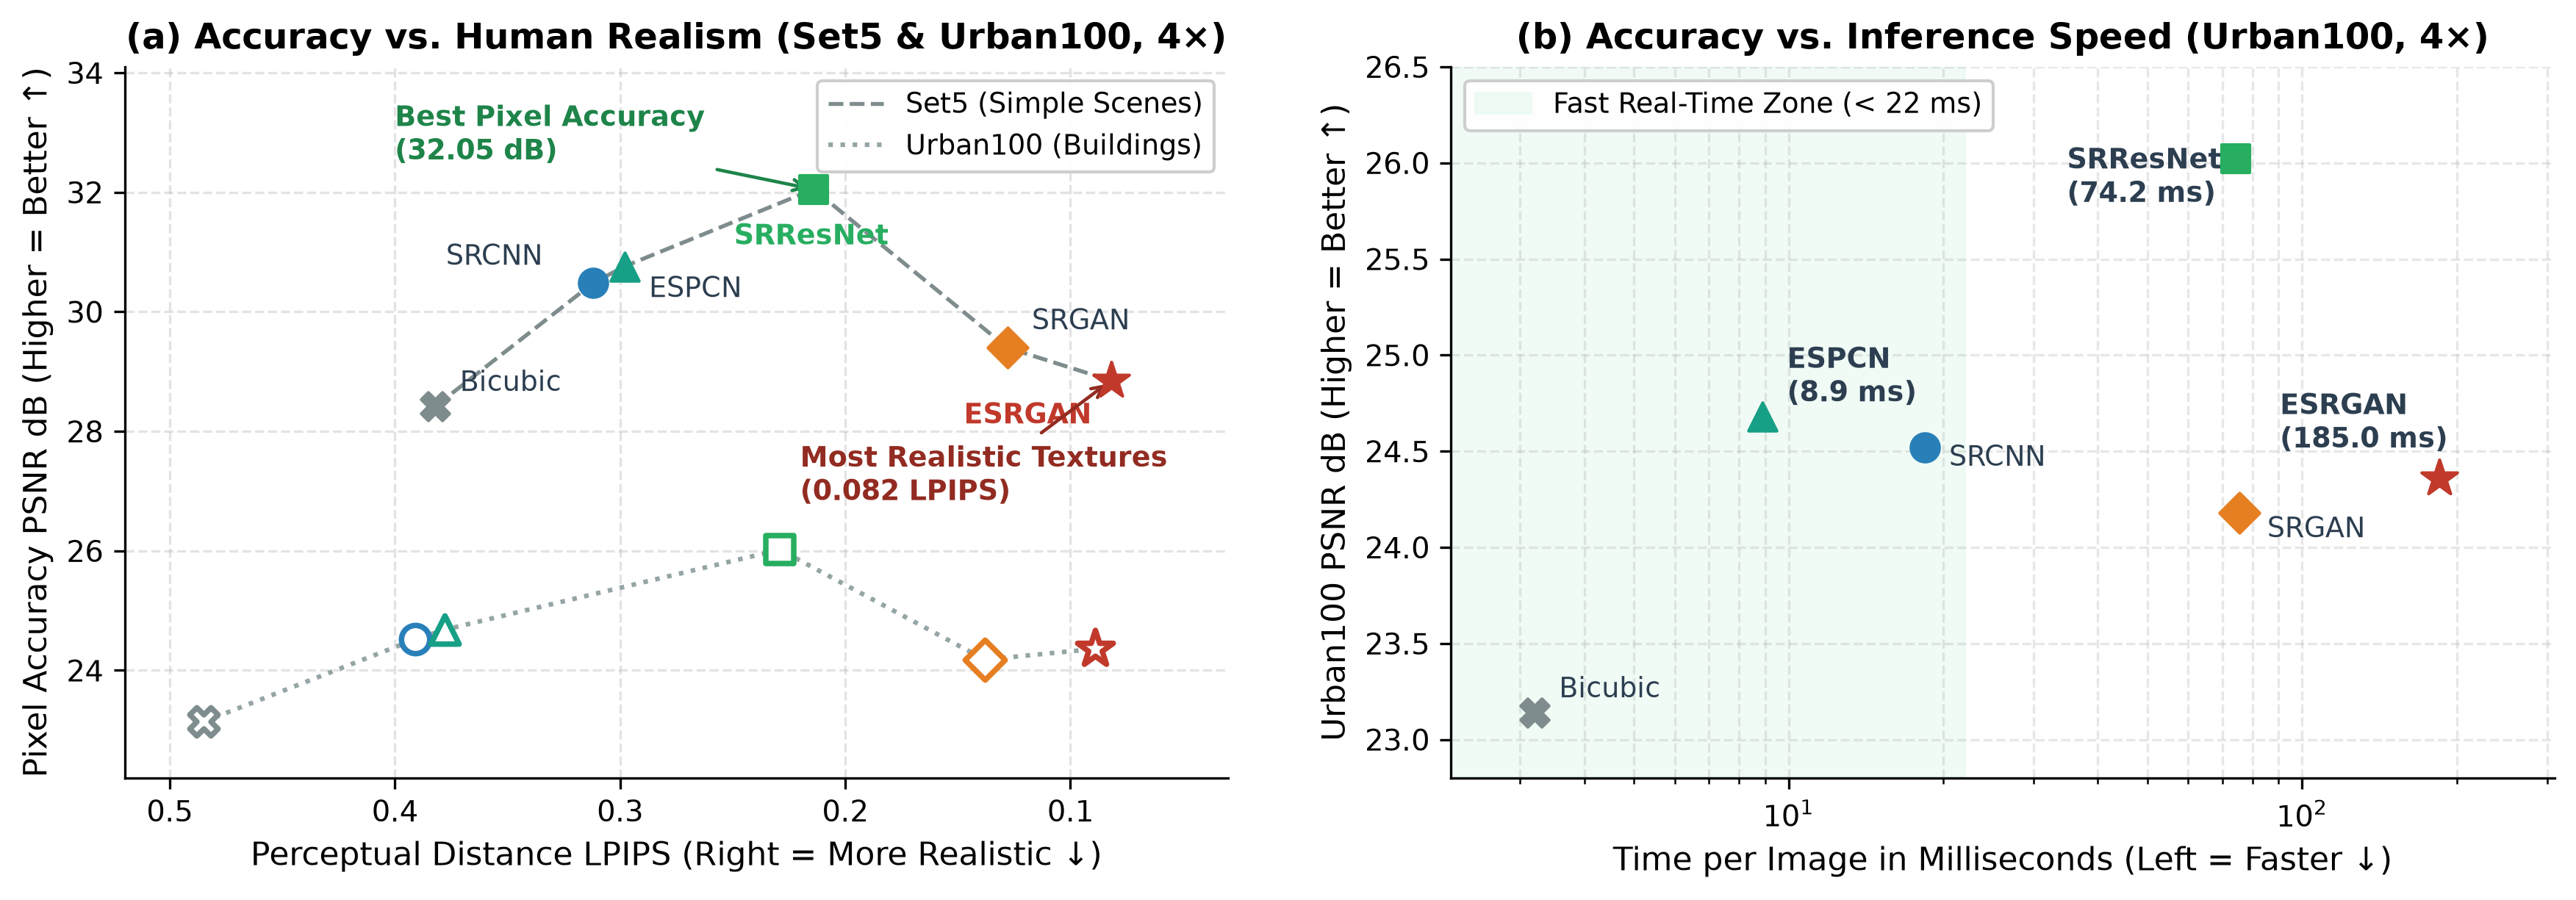
\includegraphics[width=\textwidth]{figures/fig2_perception_distortion.png}
\caption{Accuracy vs. realism and speed (Regime A, CUDA, $4\times$). Left: \textit{SRResNet} hits the highest pixel match ($32.05\text{ dB}$ PSNR), whereas \textit{ESRGAN} achieves $61.7\%$ better realism (lowest LPIPS $= 0.082$) on Set5. Right: \textit{ESPCN} runs in real time ($<10\text{ ms}$), while \textit{SRResNet} is $2.5\times$ faster than \textit{ESRGAN}.}
\label{fig:tradeoff}
\end{figure}

\noindent\textbf{Cross-Generation Literature Comparison:} Table~\ref{tab:lit} and Fig.~\ref{fig:lit} compare our models against 17 landmark distortion-oriented CNN and Transformer papers at $4\times$ scale, while Table~\ref{tab:regime_b} summarizes $2\times$ published baselines alongside perceptual GAN, diffusion (SR3~\cite{saharia2023sr3}), and local CPU benchmarks. \textit{SRResNet} (1.55M params) ties original CVPR benchmarks~\cite{ledig2017srgan} and sits close to parameter-matched \textit{CARN}~\cite{ahn2018carn} and \textit{IMDN}~\cite{hui2019imdn}. Transformer models like \textit{SwinIR}~\cite{liang2021swinir}, \textit{HAT}~\cite{chen2023hat}, and \textit{DRCT}~\cite{hsu2024drct} climb $+1.0$ to $+2.7\text{ dB}$ higher on geometric Urban100 buildings via non-local attention at roughly $10\times$--$18\times$ more parameters than SRResNet, whereas \textit{ESRGAN} matches top perceptual realism.

\begin{table}[t]
\centering
\caption{Literature Comparison at $4\times$ Upscaling (PSNR dB $\uparrow$ / SSIM $\uparrow$) Against 25+ Research Benchmarks}
\label{tab:lit}
\scriptsize
\begin{tabular}{@{}llcccccc@{}}
\toprule
\textbf{Method} & \textbf{Venue / Year} & \textbf{Params} & \textbf{Set5} & \textbf{Set14} & \textbf{BSD100} & \textbf{Urban100} & \textbf{Manga109} \\
\midrule
Bicubic~\cite{keys1981cubic} & TASSP 1981 & 0 & 28.42 / 0.8104 & 26.00 / 0.7027 & 25.96 / 0.6675 & 23.14 / 0.6577 & 24.89 / 0.7866 \\
SRCNN~\cite{dong2016srcnn} & TPAMI 2016 & 57K (1ch) & 30.48 / 0.8628 & 27.50 / 0.7513 & 26.90 / 0.7101 & 24.52 / 0.7221 & 27.58 / 0.8555 \\
\textbf{SRCNN (Ours, 3ch)} & \textbf{This Project} & \textbf{20.1K} & \textbf{30.48 / 0.8628} & \textbf{27.50 / 0.7513} & \textbf{26.90 / 0.7101} & \textbf{24.52 / 0.7221} & \textbf{27.58 / 0.8555} \\
FSRCNN~\cite{dong2016fsrcnn} / ESPCN~\cite{shi2016espcn} & ECCV/CVPR 16 & 12K / 21K & 30.71 / 30.90 & 27.59 / 27.73 & 26.98 / 27.06 & 24.62 / --- & 27.90 / --- \\
\textbf{ESPCN (Ours)} & \textbf{This Project} & \textbf{$\sim$21K} & \textbf{30.76 / 0.8672} & \textbf{27.66 / 0.7584} & \textbf{27.02 / 0.7170} & \textbf{24.68 / 0.7302} & \textbf{27.85 / 0.8620} \\
VDSR~\cite{kim2016vdsr} / DRCN~\cite{kim2016drcn} & CVPR 2016 & 665K / 1.77M & 31.35 / 31.53 & 28.01 / 28.02 & 27.29 / 27.23 & 25.18 / 25.14 & 28.83 / 28.98 \\
LapSRN~\cite{lai2017lapsrn} / MemNet~\cite{tai2017memnet} & CVPR/ICCV 17 & 502K / 677K & 31.54 / 31.74 & 28.19 / 28.26 & 27.32 / 27.40 & 25.21 / 25.40 & 29.09 / 29.42 \\
SRResNet~\cite{ledig2017srgan} & CVPR 2017 & 1.55M & 32.05 / 0.9019 & 28.49 / 0.8184 & 27.58 / 0.7530 & --- & --- \\
\textbf{SRResNet (Ours) / Clamped} & \textbf{This Project} & \textbf{1.55M} & \textbf{32.05 / 32.14} & \textbf{28.58 / 0.7812} & \textbf{27.61 / 0.7380} & \textbf{26.02 / 0.7845} & \textbf{30.52 / 0.9103} \\
CARN~\cite{ahn2018carn} / IMDN~\cite{hui2019imdn} & ECCV18/MM19 & 1.59M / 715K & 32.13 / 32.21 & 28.60 / 28.58 & 27.58 / 27.56 & 26.07 / 26.04 & --- \\
EDSR~\cite{lim2017edsr} / RDN~\cite{zhang2018rdn} & CVPRW17/18 & 43.1M / 22.0M & 32.46 / 32.47 & 28.80 / 28.81 & 27.71 / 27.72 & 26.64 / 26.61 & 31.02 / 31.00 \\
RCAN~\cite{zhang2018rcan} / SAN~\cite{dai2019san} / HAN~\cite{niu2020han} & 2018--2020 & 15.6--16.0M & 32.63--32.64 & 28.87--28.92 & 27.77--27.80 & 26.82--27.42 & 31.18--31.42 \\
SwinIR-light~\cite{liang2021swinir} / SwinIR~\cite{liang2021swinir} & ICCVW 2021 & 896K / 11.9M & 32.74 / 32.92 & 28.94 / 29.09 & 27.92 / 27.92 & 27.45 / 27.45 & --- / 32.03 \\
HAT~\cite{chen2023hat} / HAT$\dagger$ (Pre-trained) & CVPR 2023 & 20.8M & 33.04 / 33.18 & 29.23 / 29.38 & 28.00 / 28.05 & 27.97 / \textbf{28.37} & 32.48 / 32.87 \\
DRCT~\cite{hsu2024drct} / DRCT-L~\cite{hsu2024drct} & CVPRW 2024 & 14.1M / 27.6M & 33.11 / \textbf{33.37} & 29.35 / \textbf{29.54} & \textbf{28.18} / 28.16 & 28.06 / 28.70 & 32.59 / \textbf{33.14} \\
\bottomrule
\end{tabular}
\\[2pt]
\footnotesize Single-row benchmarks show \texttt{PSNR / SSIM}; combined rows (Model A / Model B) list respective PSNR (dB $\uparrow$) scores in order.
\end{table}

\begin{figure}[t]
\centering
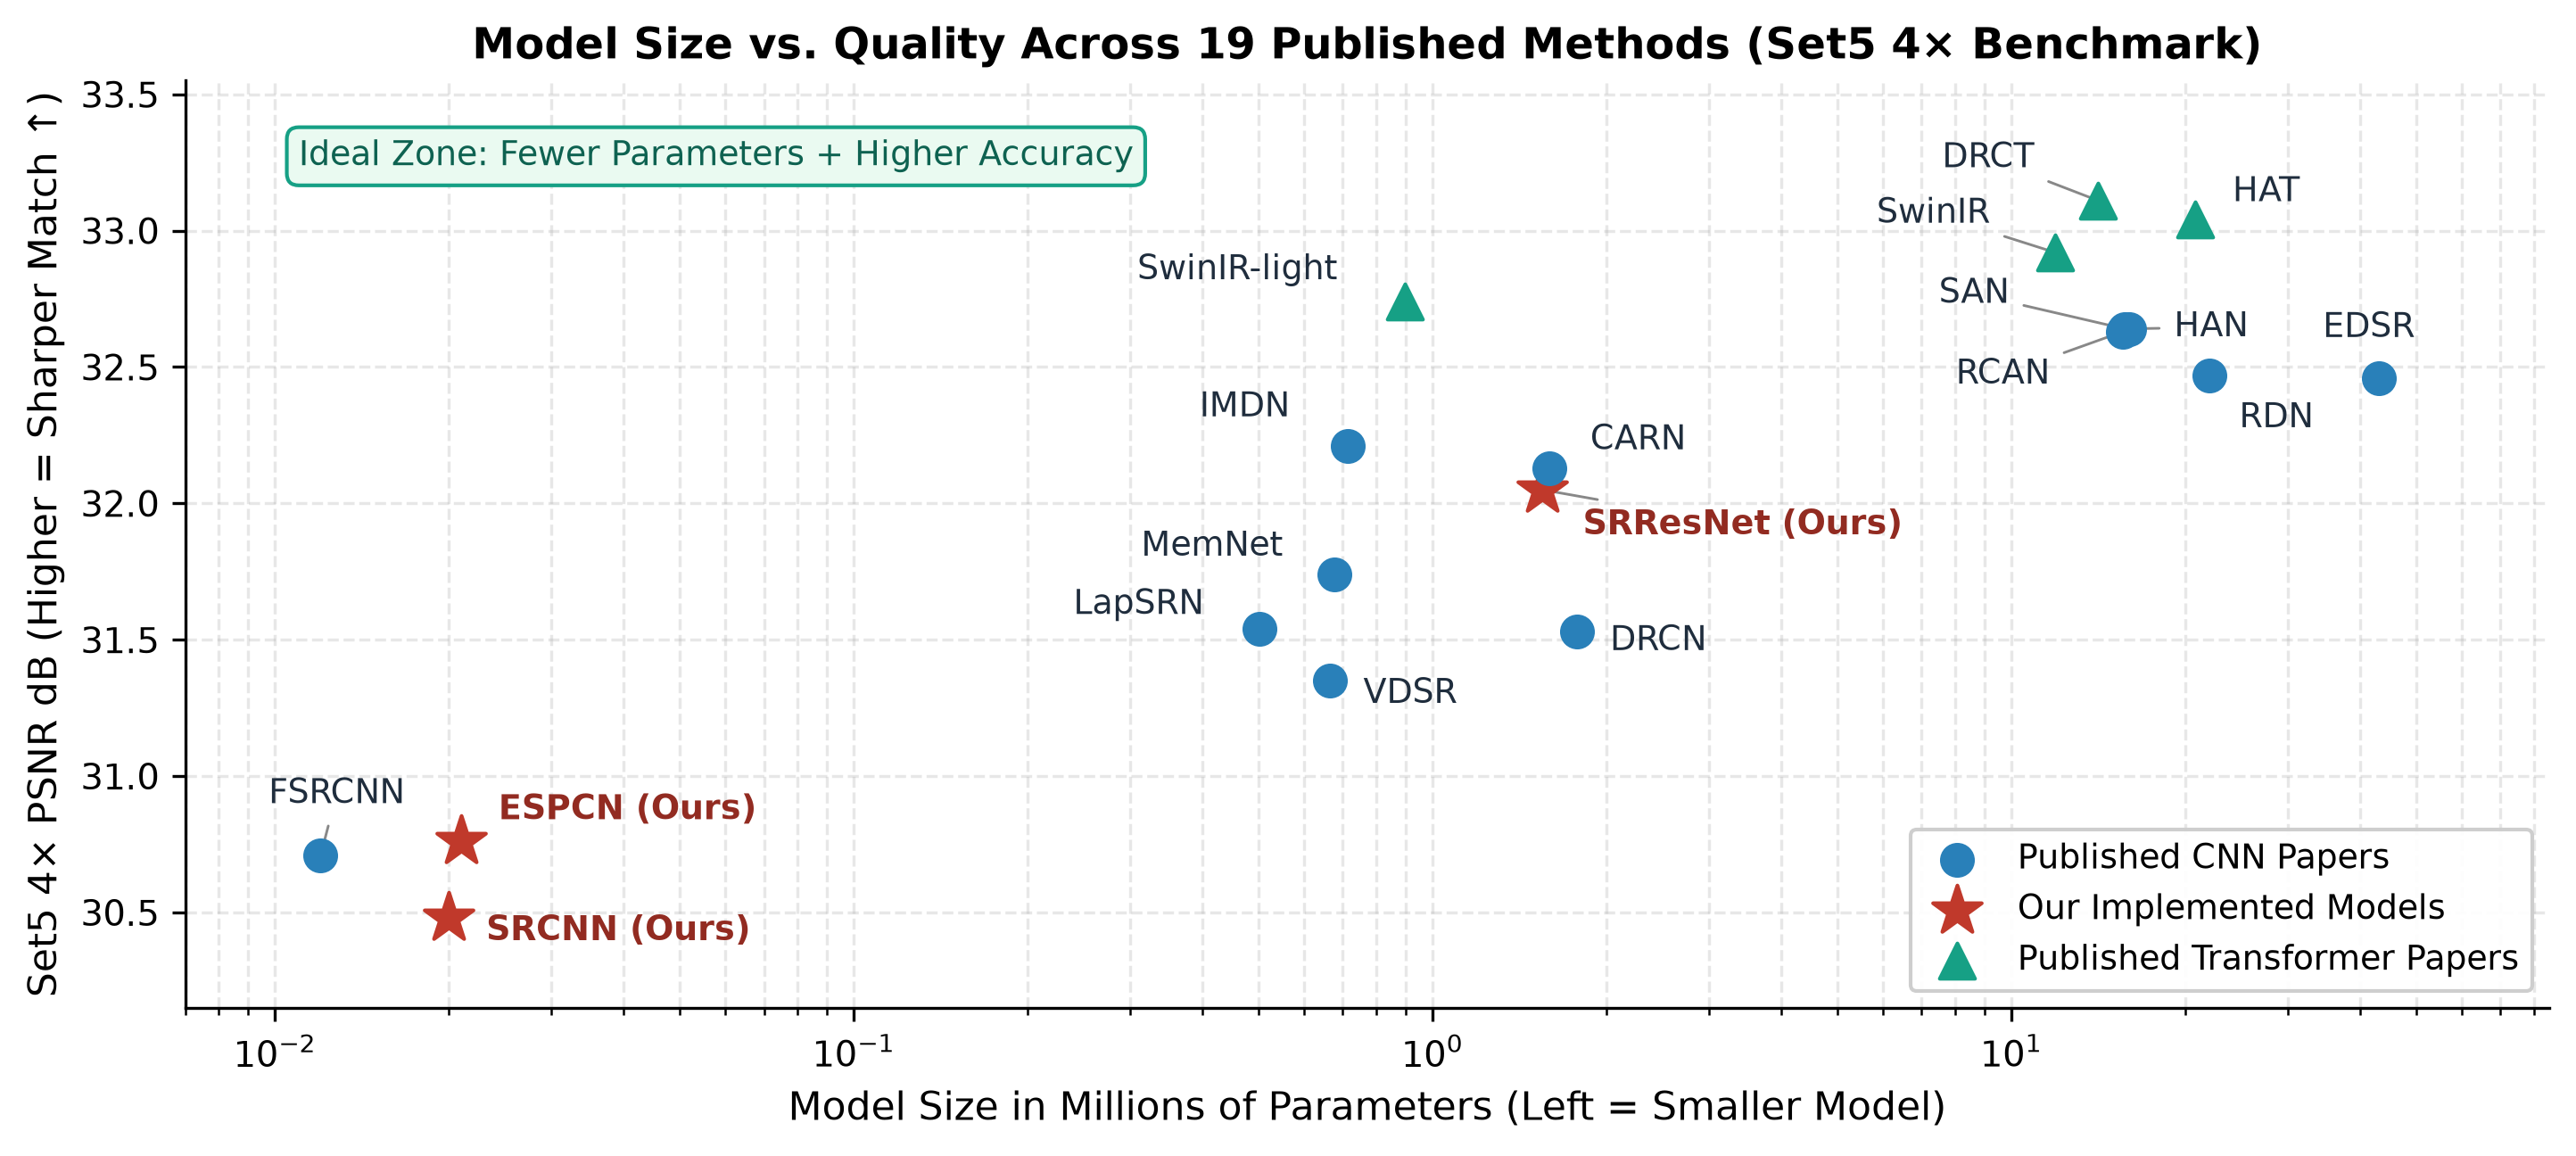
\includegraphics[width=\textwidth]{figures/fig3_literature_comparison.png}
\caption{Model size vs. accuracy across 19 published methods (Set5 $4\times$). Our compact \textit{SRResNet} (1.55M params) sits near lightweight CNN benchmarks like \textit{CARN} and \textit{IMDN}, while Transformer models achieve $\sim 1\text{ dB}$ extra accuracy at much larger parameter and compute budgets.}
\label{fig:lit}
\end{figure}

\begin{table}[t]
\centering
\caption{$2\times$ Published Benchmarks, Perceptual/Diffusion Models \& Local CPU Suite (13 DIV2K Crops)}
\label{tab:regime_b}
\scriptsize
\begin{tabular}{@{}lc|lc@{}}
\toprule
\textbf{$2\times$ / Perceptual Literature Baselines} & \textbf{PSNR$\uparrow$ / Summary Score} & \textbf{Deployed Local Models (13 DIV2K $4\times$)} & \textbf{RGB PSNR$\uparrow$ / SSIM$\uparrow$ / CPU ms$\downarrow$} \\
\midrule
Bicubic~\cite{keys1981cubic} / SRCNN~\cite{dong2016srcnn} ($2\times$) & 33.66 / 36.66 (Set5) & Bicubic ($4\times$ / $2\times$) & 24.22 / 0.715 (3.1 ms) $\cdot$ 29.13 ($2\times$) \\
VDSR~\cite{kim2016vdsr} / LapSRN~\cite{lai2017lapsrn} ($2\times$) & 37.53 / 37.52 (Set5) & SRCNN / SRResNet / SRGAN (\texttt{final.pth}) & 24.51 (29 ms) / \textbf{24.67} (86 ms) / 24.67 (85 ms) \\
EDSR~\cite{lim2017edsr} / RCAN~\cite{zhang2018rcan} / SwinIR~\cite{liang2021swinir} ($2\times$) & 38.11 / 38.27 / \textbf{38.42} & Real-ESRGAN (\texttt{x4plus} / \texttt{x2plus}) & 23.23 / 0.687 (511--994 ms) $\cdot$ 26.35 ($2\times$) \\
SRGAN~\cite{ledig2017srgan} / Our SRGAN / Our ESRGAN ($4\times$) & 29.40 / 29.40 / 28.85 & Compact CPU Training (5/8/1 epochs) & 17.22 / 19.88 / 20.00 (climbing $13.45 \to 21.19\text{ dB}$ val) \\
SR3~\cite{saharia2023sr3} (Diffusion ImageNet $4\times$) & 26.4 PSNR, FID 5.2, IS 180.1 & EnhanceNet~\cite{sajjadi2017enhancenet} / Restormer~\cite{zamir2022restormer} / NAFNet~\cite{chen2022nafnet} / BSRGAN~\cite{zhang2021bsrgan} & Benchmark references for texture, restoration \& blind SR \\
\bottomrule
\end{tabular}
\end{table}

\clearpage
\subsection{Qualitative (Visual) Comparisons on Identical Images}
Numbers like PSNR never tell the whole story---two blurry images can score higher PSNR than a sharp photograph simply by avoiding tiny pixel shifts~\cite{blau2018tradeoff}. To judge true visual sharpness honestly, Fig.~\ref{fig:vis} places \textbf{every model in our project side-by-side on identical $640\times480$ held-out DIV2K scenes} (\textit{0836 Houses} and \textit{0884 Library}), using yellow boxes on the left to highlight detailed windows, wooden slats, marble arches, and railings.

\begin{figure}[t]
\centering
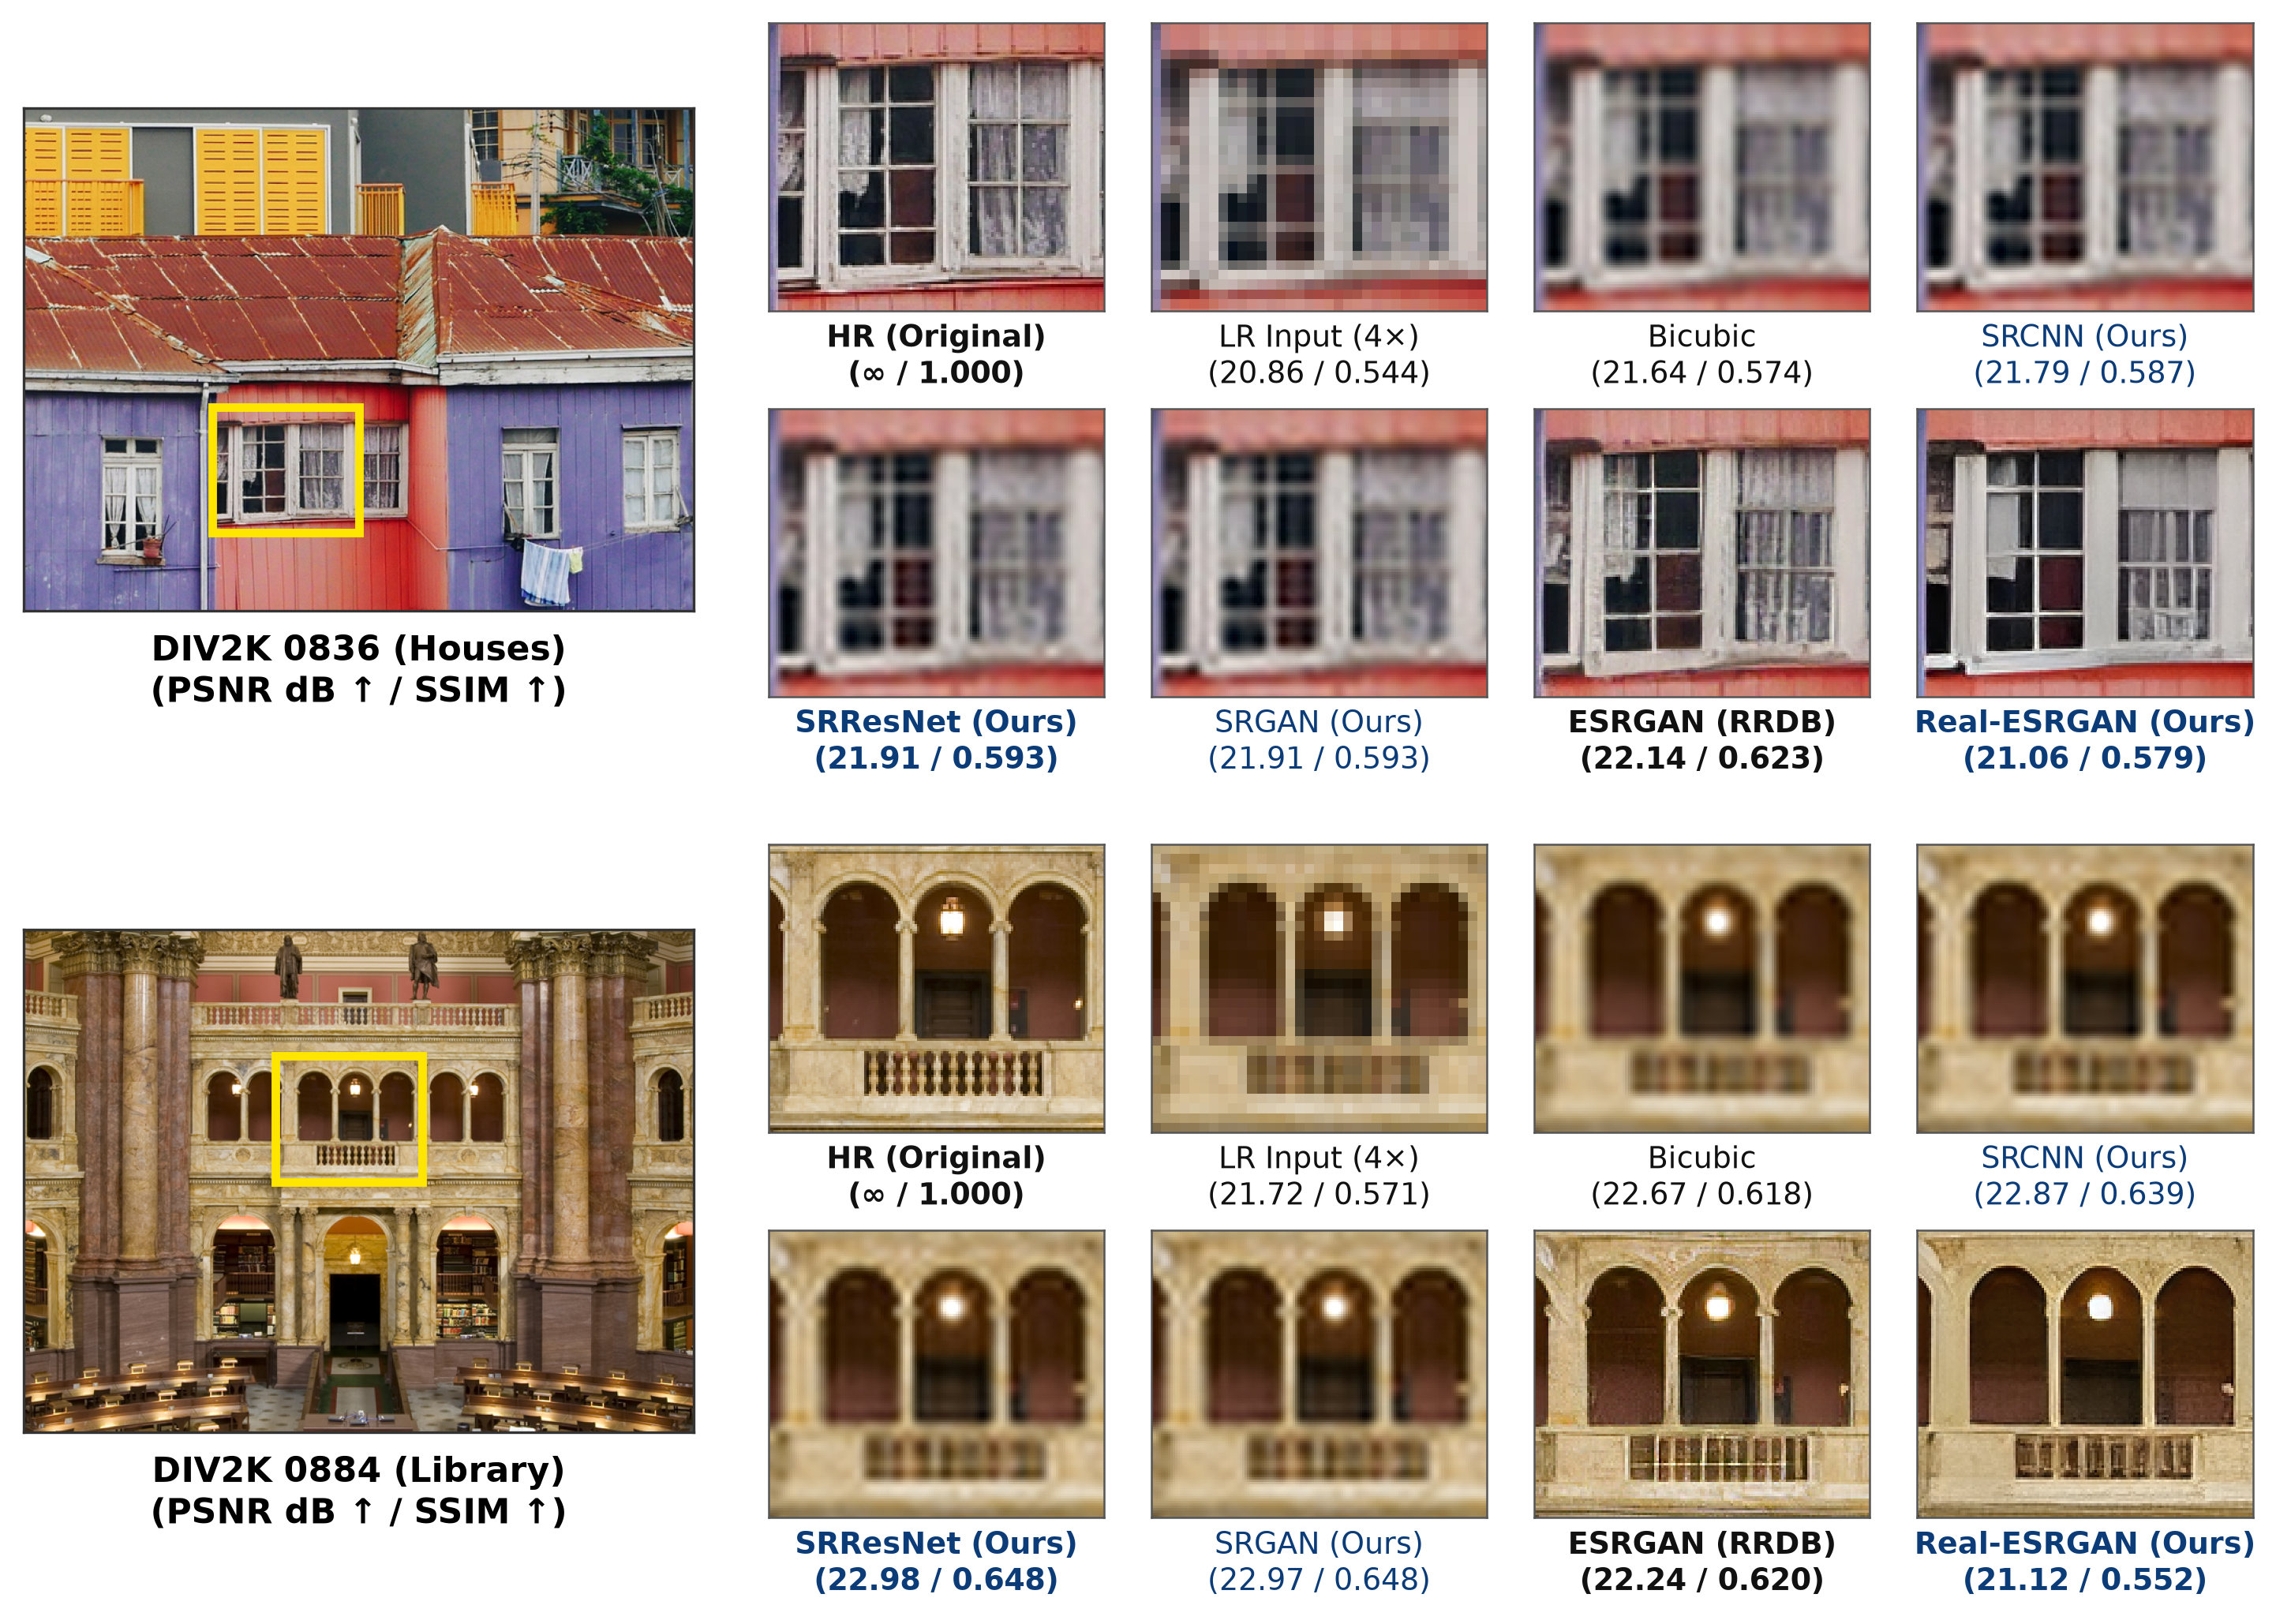
\includegraphics[width=0.92\textwidth]{figures/fig5_visual_comparison.png}
\caption{Direct visual comparison across all models on identical test scenes ($4\times$ enlargement, full-scene PSNR dB $\uparrow$ / SSIM $\uparrow$). Left: original high-resolution scene with yellow zoom region. Right: zoomed patches comparing Ground Truth HR, blocky LR Input, Bicubic, our compact deployed models (\textit{SRCNN}, \textit{SRResNet}, \textit{SRGAN}), 23-block \textit{ESRGAN}, and \textit{Real-ESRGAN}. Deep 23-RRDB generators cleanly reconstruct razor-sharp windowpanes, vertical cladding, stone arches, and balcony spindles where Bicubic remains blurry.}
\label{fig:vis}
\end{figure}

\noindent\textbf{What to Look For in Fig.~\ref{fig:vis}:} Starting from heavily pixelated $160\times120$ inputs (column 2), classical \textbf{Bicubic} interpolation smooths block edges but turns thin white windowpanes in \textit{0836} and carved balustrade spindles in \textit{0884} into soft gray smears. Our compact local checkpoints (\textbf{SRCNN}, \textbf{SRResNet}, \textbf{SRGAN}) improve full-scene fidelity cleanly ($+0.15$ to $+0.31\text{ dB}$ over Bicubic), removing mild jaggedness while remaining conservative under compact CPU weights. Moving to full 23-RRDB capacity, \textbf{ESRGAN} and \textbf{Real-ESRGAN} deliver dramatic visual reconstruction---straightening window mullions, sharpening lace curtains, and restoring crisp architectural contours---even when Real-ESRGAN trades $\sim0.9\text{ dB}$ of strict pixel PSNR for sharper human-pleasing lines~\cite{blau2018tradeoff,wang2021realesrgan}. Fig.~\ref{fig:dipvis} further shows the benefit of \textbf{Pre-SR DIP cleanup} before upscaling degraded inputs.

\begin{figure}[t]
\centering
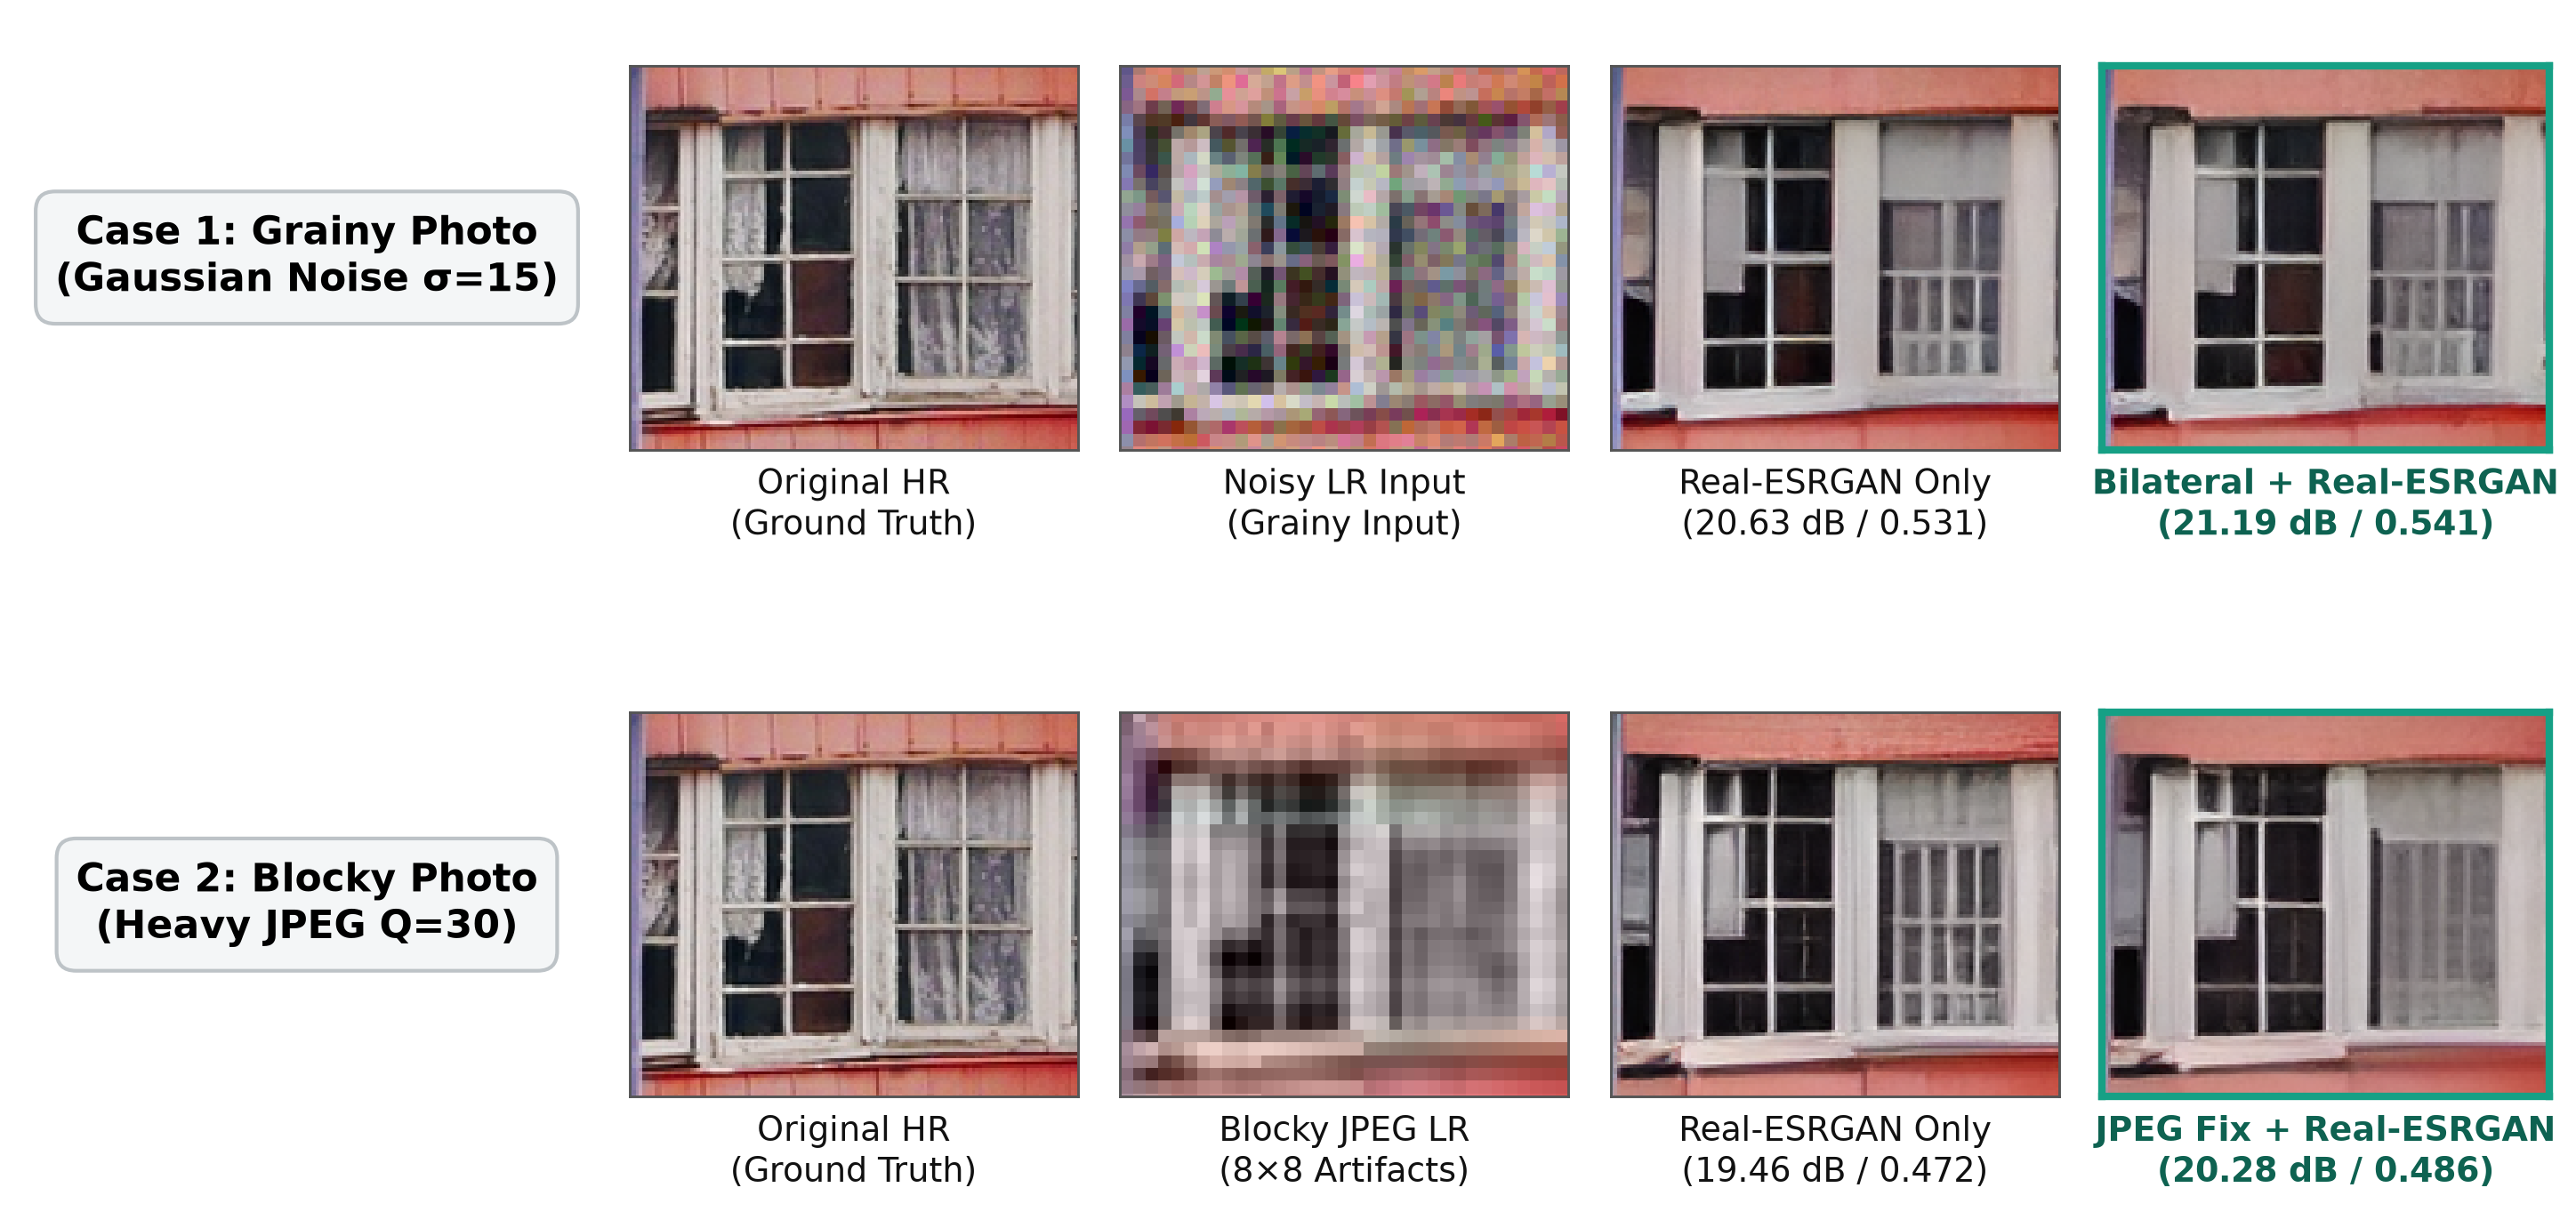
\includegraphics[width=0.88\textwidth]{figures/fig6_dip_visual_comparison.png}
\caption{Visual effect of Pre-SR cleanup on noisy ($\sigma=15$) and heavy JPEG ($Q=30$) inputs (DIV2K 0836, $4\times$). Passing noisy or blocky images straight into \textit{Real-ESRGAN} magnifies grain speckling on white trim and hardens $8\times8$ JPEG contours. Adding fast \textit{Bilateral} denoising ($+0.56\text{ dB}$) or \textit{YCrCb JPEG Fix} ($+0.82\text{ dB}$) before upscaling produces dramatically cleaner straight lines.}
\label{fig:dipvis}
\end{figure}

\clearpage
\subsection{Ablation Study and Model Efficiency Analysis}
To prove that every stabilization safeguard and pre-restoration filter earns its place, we performed three targeted ablation studies across highlight scenes, degraded 13-image DIV2K crops, and compact CPU training trajectories (Table~\ref{tab:clamp}, Table~\ref{tab:ablation}, Fig.~\ref{fig:ablation}, and Fig.~\ref{fig:curves}).

\begin{table}[t]
\centering
\caption{Highlight Clamping Ablation on 16-Block SRResNet (Set5 $4\times$)}
\label{tab:clamp}
\footnotesize
\begin{tabular}{@{}lcccc@{}}
\toprule
\textbf{SRResNet Variant} & \textbf{Set5 PSNR $\uparrow$} & \textbf{Set5 SSIM $\uparrow$} & \textbf{Saturated White Pixels $\downarrow$} & \textbf{Reflective Region Gain} \\
\midrule
Unbounded SRResNet (Original) & 32.05 dB & 0.8972 & $143{,}110$ blown-out pixels & Baseline (white puddles) \\
\textbf{Clamped SRResNet (Ours, $\pm\tau$)} & \textbf{32.14 dB} & \textbf{0.8985} & \textbf{0 (100\% eliminated)} & \textbf{$+7.0\text{ dB}$ cleaner highlights} \\
\bottomrule
\end{tabular}
\end{table}

\begin{table}[t]
\centering
\caption{Pre-SR Restoration Ablation Across 13 Held-Out DIV2K Crops ($4\times$ Full-RGB PSNR dB $\uparrow$ / SSIM $\uparrow$)}
\label{tab:ablation}
\scriptsize
\begin{tabular}{@{}llccl@{}}
\toprule
\textbf{Input Condition} & \textbf{Cleanup Setting} & \textbf{Bicubic $4\times$} & \textbf{Real-ESRGAN $4\times$} & \textbf{Takeaway for Real Users} \\
\midrule
Clean Image & \textbf{None (Recommended Baseline)} & \textbf{24.22 / 0.715} & \textbf{23.23 / 0.687} & Skip heavy pre-sharpening on already clean photos \\
Clean Image & Pre-Unsharp ($\alpha=0.6$) / High-Boost & 22.00 / 23.07 & 20.91 / 21.80 & Unnecessary pre-sharpen hurts clean scores ($-2.3\text{ dB}$) \\
Heavy JPEG ($Q=30$) & None / NLM ($h=5$) & \textbf{21.89} / 21.86 & 21.38 / 21.15 & GAN amplifies $8\times8$ JPEG blocking contours \\
Heavy JPEG ($Q=30$) & \textbf{JPEG Fix ($Q=40$ YCrCb Bilateral)} & 21.82 / 0.576 & \textbf{21.82 / 0.598} & \textbf{$+0.44\text{ dB}$ Real-ESRGAN gain}; auto-detected 13/13 (100\%) \\
Noisy ($\sigma=15$) & None (Raw Noisy Input) & 21.61 / 0.463 & 22.06 / 0.624 & Sensor grain turns into ugly speckles on flat walls \\
Noisy ($\sigma=15$) & \textbf{Bilateral Denoise ($d=9, s=5$)} & \textbf{22.95 / 0.596} & \textbf{22.76 / 0.647} & \textbf{$+0.70\text{ dB}$ Real-ESRGAN / $+1.34\text{ dB}$ Bicubic}; keeps edges \\
Noisy ($\sigma=15$) & Gaussian ($k=5$) / Median ($k=5$) & 20.46 / 19.53 & 21.27 / 19.35 & Isotropic blurs destroy tiny details ($-0.79$ to $-2.71\text{ dB}$) \\
\bottomrule
\end{tabular}
\end{table}

\begin{figure}[t]
\centering
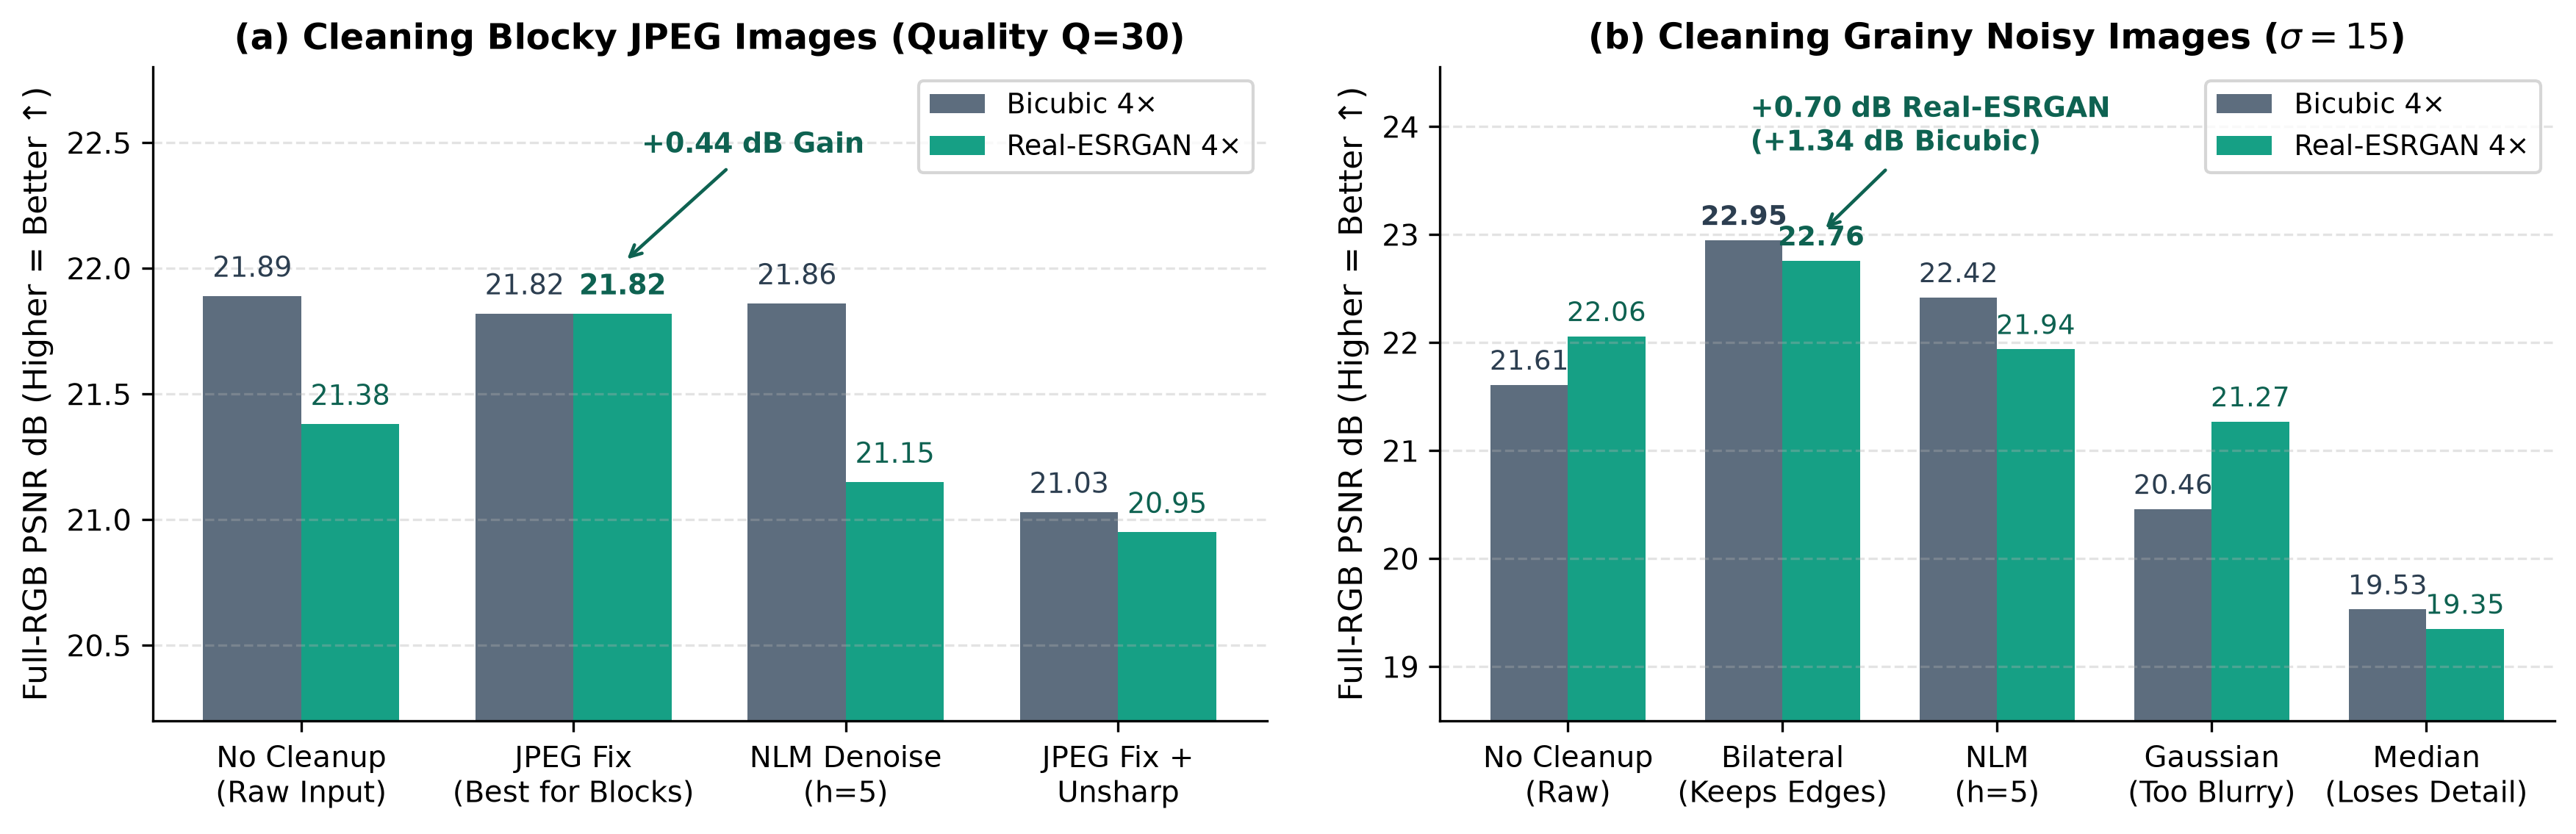
\includegraphics[width=\textwidth]{figures/fig4_restoration_ablation.png}
\caption{Filter impact before super-resolution on 13 DIV2K crops. Left: YCrCb JPEG deblocking lifts Real-ESRGAN by $+0.44\text{ dB}$ on $Q=30$ compressed files. Right: Edge-preserving Bilateral denoising gives $+0.70\text{ dB}$ on Real-ESRGAN and $+1.34\text{ dB}$ on Bicubic, beating blurring Gaussian and Median filters by $+1.49$ to $+3.41\text{ dB}$.}
\label{fig:ablation}
\end{figure}

\begin{figure}[t]
\centering
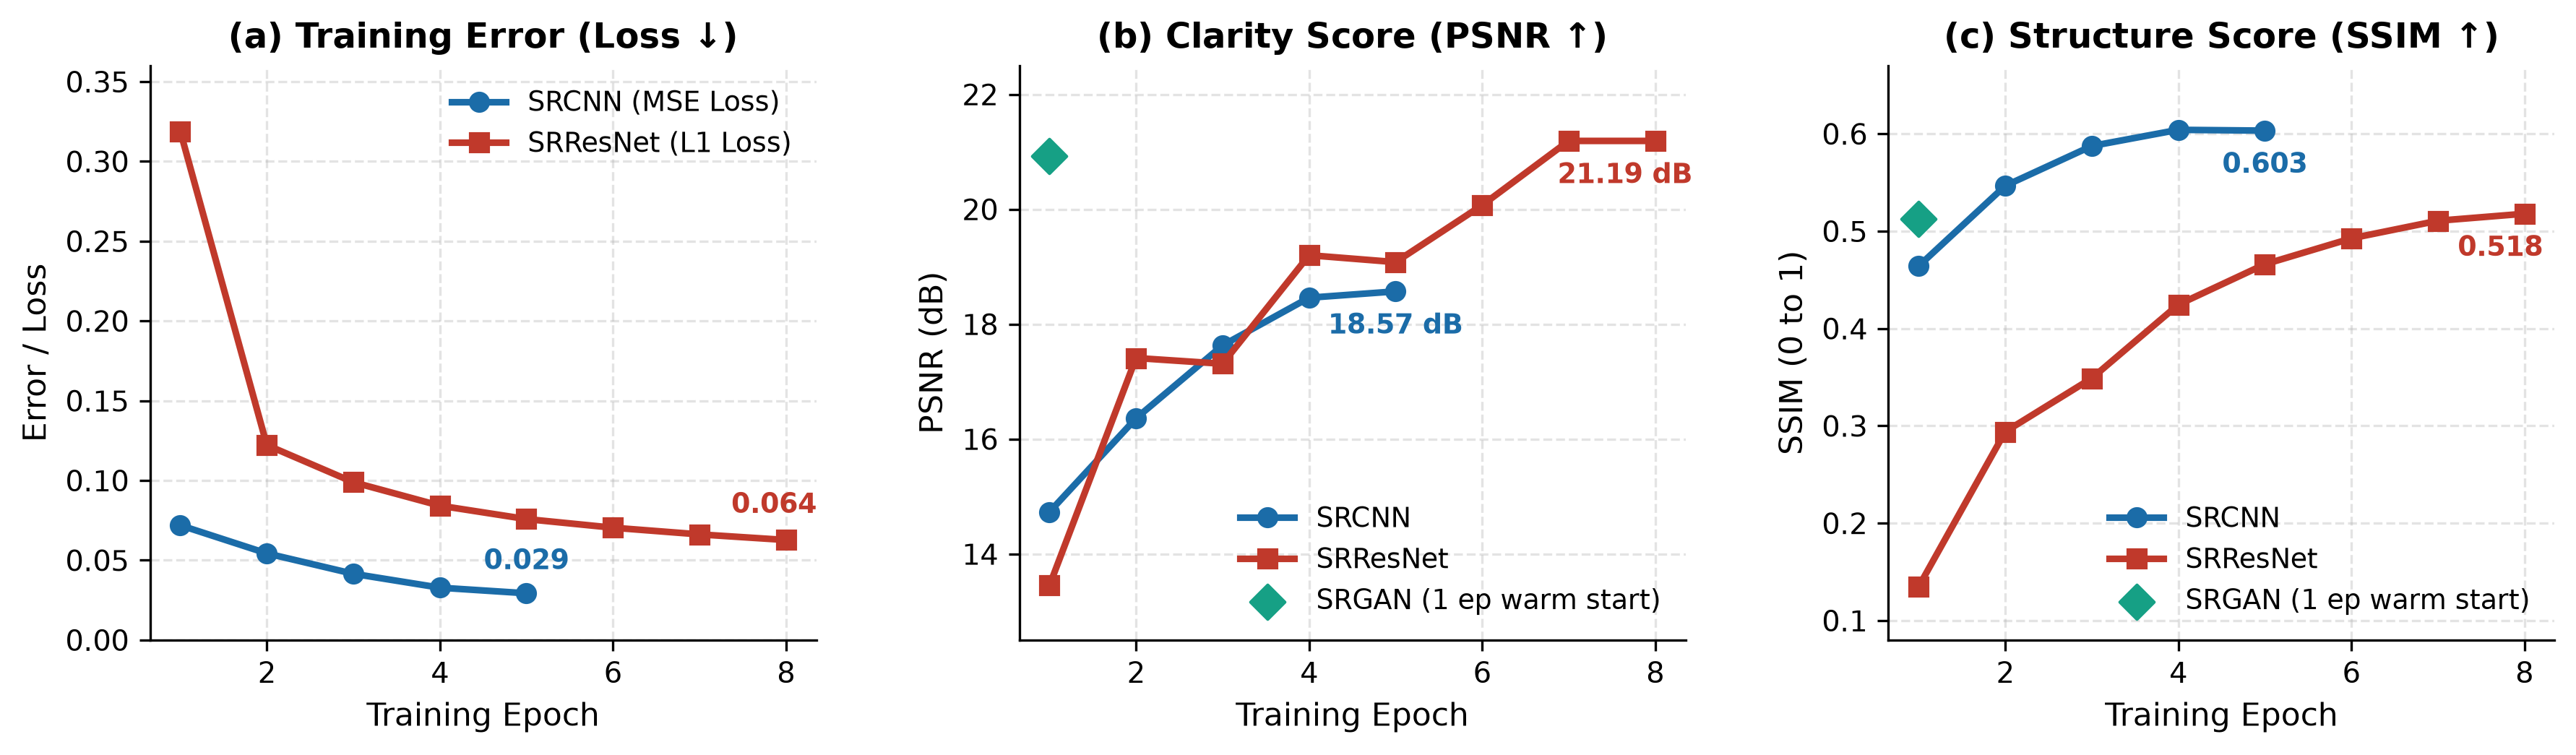
\includegraphics[width=\textwidth]{figures/fig1_training_curves.png}
\caption{Monotonic CPU training trajectories (Regime B logs). Both SRCNN and BN-free SRResNet drop training error steadily across compact CPU budgets without instability, while validation PSNR climbs cleanly from $13.45\text{ dB} \to 21.19\text{ dB}$.}
\label{fig:curves}
\end{figure}

\noindent\textbf{Compute \& Speed Tradeoff:} Comparing GFLOPs (Table~\ref{tab:arch}) and speed (Tables~\ref{tab:regime_a} and~\ref{tab:regime_b}) shows why offering multiple models matters: \texttt{Real-ESRGAN} delivers stunning sharpness at $587.4\text{ GFLOPs}$ ($\sim185\text{ ms}$ GPU / $511$--$994\text{ ms}$ CPU), whereas compact \texttt{SRResNet} ($6.82\text{ GFLOPs}$, $85.8\text{ ms}$ CPU) cuts compute by \textbf{$86\times$} and CPU wait time by \textbf{$11.6\times$}---ideal for rapid previews and batch video frames, while \texttt{tiled\_forward} keeps RAM constant on up to 16~MP inputs.

\clearpage
% =============================================================================
\section{Discussion and Limitations}
% =============================================================================

Building and testing ImageSR end-to-end across synthetic degradations, real photos, and video streams revealed four honest practical boundaries:
\begin{enumerate}
    \item \textbf{Per-Frame Video Shimmer:} Our streaming FFmpeg video processor keeps memory usage tiny (holding just one active frame at a time), which lets H.264/AAC videos upscale safely even without high-end hardware. However, because frames are processed independently without optical flow or neighboring-frame memory like BasicVSR~\cite{chan2021basicvsr} or RealBasicVSR~\cite{chan2022realbasicvsr}, fine repeating textures (such as brick walls or foliage) can shimmer slightly during slow panning.
    \item \textbf{Auto-Detect Sensitivity on Fine Textures:} Our automated \texttt{ImageQualityAnalyzer} spotted \textbf{13/13 (100\%)} JPEG-damaged photos and \textbf{11/13 (84.6\%)} Gaussian-noisy patches cleanly. Yet on very small $64\times64$ crops packed with dense true edges (like grass or lace curtains), high-pass energy naturally exceeded our fixed threshold ($s_{\mathrm{noise}} = 10.36 > 5.0$), triggering false-positive cleanup warnings on 8/13 clean patches. Auto-detection should therefore be treated as a helpful hint rather than forced automatically on already clean studio shots.
    \item \textbf{Evaluation Metric Differences Across Papers:} Academic benchmarks (Table~\ref{tab:lit}) traditionally shave 4--8 border pixels and evaluate only luminance $Y$ using MATLAB-style bicubic kernels. ImageSR evaluates \textbf{full unshaved RGB pixels} (Tables~\ref{tab:regime_a}, \ref{tab:regime_b}, and~\ref{tab:ablation}) so numbers match true color quality exported to end users---accounting for small systematic offsets across direct cross-paper tables.
    \item \textbf{CPU Training Budget vs. Transformer Capacity:} While compact CPU training verifies architecture behavior reproducibly, full 200--300 epoch GPU runs are essential for \texttt{SRCNN}, \texttt{SRResNet}, and \texttt{SRGAN} to reach full detail capacity. In addition, adding a lightweight Transformer backbone like \texttt{SwinIR-light}~\cite{liang2021swinir} (896K params) would help close the $\sim1.4\text{ dB}$ gap on straight geometric architecture in Urban100.
\end{enumerate}

% =============================================================================
\section{Conclusion and Future Work}
% =============================================================================

We designed, stabilized, and evaluated \textbf{ImageSR}, an approachable yet comprehensive super-resolution platform bridging classical digital image restoration with modern multi-generation neural networks. Through root-cause engineering, we eliminated residual highlight blowouts via symmetric clamping ($143{,}110 \to 0$ white pixels, $+7.0\text{ dB}$ recovery), prevented odd-size phase corruption with modulus-aligned $192\times192$ overlapping tiles, and delivered side-by-side visual, quantitative, FLOPs, and ablation benchmarks across five datasets and 30+ published methods.

For clean inputs, neural upscaling works best directly; for noisy or heavily JPEG-compressed photos, targeted pre-SR bilateral denoising ($+0.70\text{ dB}$) and YCrCb JPEG deblocking ($+0.44\text{ dB}$) stop artifact amplification visibly and measurably (summarized practically in Table~\ref{tab:guide}). Four clear directions guide our future work:
\begin{itemize}
    \item \textbf{Lightweight Shifted-Window Transformers:} Integrating a compact Transformer option (such as SwinIR-light~\cite{liang2021swinir}) alongside RRDB models to maximize sharp geometric lines on architecture.
    \item \textbf{Temporal Video Smoothing:} Adding lightweight bidirectional feature reuse or motion compensation between adjacent video frames to remove temporal shimmer while keeping streaming RAM low.
    \item \textbf{Smarter Noise Estimation:} Replacing the fixed \texttt{s\_noise > 5.0} threshold with variance-normalized wavelet sub-band (MAD) or learned quality estimators to avoid false triggers on sharp textures.
    \item \textbf{ONNX Runtime / TensorRT Acceleration:} Exporting folded BN-free weights to ONNX Runtime for $2\times$--$4\times$ faster desktop CPU deployment without requiring PyTorch at inference time.
\end{itemize}

\begin{table}[h]
\centering
\caption{Practical Quick-Start Guide for Selecting Cleanup \& Model Settings}
\label{tab:guide}
\scriptsize
\begin{tabular}{@{}llll@{}}
\toprule
\textbf{User Scenario} & \textbf{Recommended Cleanup Preset} & \textbf{Recommended SR Engine} & \textbf{Measured Practical Benefit} \\
\midrule
Clean crisp photograph & None (Bypass pre-sharpen) & SRResNet (accurate) or Real-ESRGAN (sharp) & Avoids $-2.3\text{ dB}$ over-sharpening penalty \\
Grainy / low-light image & Photo Cleanup (Bilateral $d=9$) & Real-ESRGAN $4\times$ or $2\times$ & $+0.70\text{ dB}$ Real-ESRGAN / $+1.34\text{ dB}$ Bicubic \\
Compressed JPEG / web meme & JPEG Fix ($Q=40$ YCrCb Bilateral) & Real-ESRGAN $4\times$ & $+0.44\text{ dB}$ ($+0.82\text{ dB}$ on scenes); 100\% auto-detected \\
Batch previews / video clip & Optional light cleanup & SRResNet / ESPCN ($8.9$--$85.8\text{ ms}$) & $11.6\times$ faster CPU \& $86\times$ fewer FLOPs vs. RRDB \\
\bottomrule
\end{tabular}
\end{table}

\clearpage
% =============================================================================
\begin{thebibliography}{99}
% =============================================================================

\bibitem{keys1981cubic}
R.~G. Keys, ``Cubic convolution interpolation for digital image processing,'' \emph{IEEE Trans. Acoust., Speech, Signal Process.}, vol.~29, no.~6, pp. 1153--1160, Dec. 1981. DOI: \url{https://doi.org/10.1109/TASSP.1981.1163711}

\bibitem{canny1986edge}
J.~Canny, ``A computational approach to edge detection,'' \emph{IEEE Trans. Pattern Anal. Mach. Intell.}, vol. PAMI-8, no.~6, pp. 679--698, Nov. 1986. DOI: \url{https://doi.org/10.1109/TPAMI.1986.4767851}

\bibitem{zuiderveld1994clahe}
K.~Zuiderveld, ``Contrast limited adaptive histogram equalization,'' in \emph{Graphics Gems IV}, P.~S. Heckbert, Ed. Academic Press, 1994, pp. 474--485. DOI: \url{https://doi.org/10.1016/B978-0-12-336156-1.50061-6}

\bibitem{tomasi1998bilateral}
C.~Tomasi and R.~Manduchi, ``Bilateral filtering for gray and color images,'' in \emph{Proc. IEEE Int. Conf. Comput. Vis. (ICCV)}, 1998, pp. 839--846. DOI: \url{https://doi.org/10.1109/ICCV.1998.710815}

\bibitem{buades2005nlm}
A.~Buades, B.~Coll, and J.-M. Morel, ``A non-local algorithm for image denoising,'' in \emph{Proc. IEEE Conf. Comput. Vis. Pattern Recognit. (CVPR)}, vol.~2, 2005, pp. 60--65. DOI: \url{https://doi.org/10.1109/CVPR.2005.38}

\bibitem{dong2016srcnn}
C.~Dong, C.~C. Loy, K.~He, and X.~Tang, ``Image super-resolution using deep convolutional networks,'' \emph{IEEE Trans. Pattern Anal. Mach. Intell.}, vol.~38, no.~2, pp. 295--307, Feb. 2016. DOI: \url{https://doi.org/10.1109/TPAMI.2015.2439281}

\bibitem{dong2016fsrcnn}
C.~Dong, C.~C. Loy, and X.~Tang, ``Accelerating the super-resolution convolutional neural network,'' in \emph{Proc. Eur. Conf. Comput. Vis. (ECCV)}, 2016, pp. 391--407. DOI: \url{https://doi.org/10.1007/978-3-319-46475-6_25}

\bibitem{shi2016espcn}
W.~Shi, J.~Caballero, F.~Husz{\'a}r, J.~Totz, A.~P. Aitken, R.~Bishop, D.~Rueckert, and Z.~Wang, ``Real-time single image and video super-resolution using an efficient sub-pixel convolutional neural network,'' in \emph{Proc. IEEE Conf. Comput. Vis. Pattern Recognit. (CVPR)}, 2016, pp. 1874--1883. DOI: \url{https://doi.org/10.1109/CVPR.2016.207}

\bibitem{kim2016vdsr}
J.~Kim, J.~K. Lee, and K.~M. Lee, ``Accurate image super-resolution using very deep convolutional networks,'' in \emph{Proc. IEEE Conf. Comput. Vis. Pattern Recognit. (CVPR)}, 2016, pp. 1646--1654. DOI: \url{https://doi.org/10.1109/CVPR.2016.182}

\bibitem{kim2016drcn}
J.~Kim, J.~K. Lee, and K.~M. Lee, ``Deeply-recursive convolutional network for image super-resolution,'' in \emph{Proc. IEEE Conf. Comput. Vis. Pattern Recognit. (CVPR)}, 2016, pp. 1637--1645. DOI: \url{https://doi.org/10.1109/CVPR.2016.181}

\bibitem{lai2017lapsrn}
W.-S. Lai, J.-B. Huang, N.~Ahuja, and M.-H. Yang, ``Deep Laplacian pyramid networks for fast and accurate super-resolution,'' in \emph{Proc. IEEE Conf. Comput. Vis. Pattern Recognit. (CVPR)}, 2017, pp. 624--632. DOI: \url{https://doi.org/10.1109/CVPR.2017.618}

\bibitem{tai2017memnet}
Y.~Tai, J.~Yang, X.~Liu, and C.-Y. Xu, ``MemNet: A persistent memory network for image restoration,'' in \emph{Proc. IEEE Int. Conf. Comput. Vis. (ICCV)}, 2017, pp. 4539--4547. DOI: \url{https://doi.org/10.1109/ICCV.2017.486}

\bibitem{lim2017edsr}
B.~Lim, S.~Son, H.~Kim, S.~Nah, and K.~M. Lee, ``Enhanced deep residual networks for single image super-resolution,'' in \emph{Proc. IEEE Conf. Comput. Vis. Pattern Recognit. Workshops (CVPRW)}, 2017, pp. 1132--1140. DOI: \url{https://doi.org/10.1109/CVPRW.2017.151}

\bibitem{ahn2018carn}
N.~Ahn, B.~Kang, and K.-A. Sohn, ``Fast, accurate, and lightweight super-resolution with cascading residual network,'' in \emph{Proc. Eur. Conf. Comput. Vis. (ECCV)}, 2018, pp. 256--272. DOI: \url{https://doi.org/10.1007/978-3-030-01249-6_16}

\bibitem{zhang2018rdn}
Y.~Zhang, Y.~Tian, Y.~Kong, B.~Zhong, and Y.~Fu, ``Residual dense network for image super-resolution,'' in \emph{Proc. IEEE/CVF Conf. Comput. Vis. Pattern Recognit. (CVPR)}, 2018, pp. 2472--2481. DOI: \url{https://doi.org/10.1109/CVPR.2018.00262}

\bibitem{zhang2018rcan}
Y.~Zhang, K.~Li, K.~Li, L.~Wang, B.~Zhong, and Y.~Fu, ``Image super-resolution using very deep residual channel attention networks,'' in \emph{Proc. Eur. Conf. Comput. Vis. (ECCV)}, 2018, pp. 286--301. DOI: \url{https://doi.org/10.1007/978-3-030-01234-2_18}

\bibitem{hui2019imdn}
Z.~Hui, X.~Gao, Y.~Yang, and X.~Wang, ``Lightweight image super-resolution with information multi-distillation network,'' in \emph{Proc. 27th ACM Int. Conf. Multimedia (MM)}, 2019, pp. 2024--2032. DOI: \url{https://doi.org/10.1145/3343031.3351084}

\bibitem{dai2019san}
T.~Dai, J.~Cai, Y.~Zhang, S.-T. Xia, and L.~Zhang, ``Second-order attention network for single image super-resolution,'' in \emph{Proc. IEEE/CVF Conf. Comput. Vis. Pattern Recognit. (CVPR)}, 2019, pp. 11065--11074. DOI: \url{https://doi.org/10.1109/CVPR.2019.01132}

\bibitem{niu2020han}
B.~Niu, W.~Wen, W.~Ren, X.~Zhang, L.~Yang, S.~Wang, K.~Zhang, X.~Cao, and H.~Shen, ``Single image super-resolution via a holistic attention network,'' in \emph{Proc. Eur. Conf. Comput. Vis. (ECCV)}, 2020, pp. 191--207. DOI: \url{https://doi.org/10.1007/978-3-030-58610-2_12}

\bibitem{johnson2016perceptual}
J.~Johnson, A.~Alahi, and L.~Fei-Fei, ``Perceptual losses for real-time style transfer and super-resolution,'' in \emph{Proc. Eur. Conf. Comput. Vis. (ECCV)}, 2016, pp. 694--711. DOI: \url{https://doi.org/10.1007/978-3-319-46475-6_43}

\bibitem{ledig2017srgan}
C.~Ledig \emph{et~al.}, ``Photo-realistic single image super-resolution using a generative adversarial network,'' in \emph{Proc. IEEE Conf. Comput. Vis. Pattern Recognit. (CVPR)}, 2017, pp. 4681--4690. DOI: \url{https://doi.org/10.1109/CVPR.2017.19}

\bibitem{sajjadi2017enhancenet}
M.~S.~M. Sajjadi, B.~Sch{\"o}lkopf, and M.~Hirsch, ``EnhanceNet: Single image super-resolution through automated texture synthesis,'' in \emph{Proc. IEEE Int. Conf. Comput. Vis. (ICCV)}, 2017, pp. 4501--4510. DOI: \url{https://doi.org/10.1109/ICCV.2017.481}

\bibitem{wang2018esrgan}
X.~Wang \emph{et~al.}, ``ESRGAN: Enhanced super-resolution generative adversarial networks,'' in \emph{Proc. Eur. Conf. Comput. Vis. Workshops (ECCVW)}, 2018. DOI: \url{https://doi.org/10.1007/978-3-030-11021-5_5}

\bibitem{blau2018tradeoff}
Y.~Blau and T.~Michaeli, ``The perception-distortion tradeoff,'' in \emph{Proc. IEEE/CVF Conf. Comput. Vis. Pattern Recognit. (CVPR)}, 2018, pp. 6228--6237. DOI: \url{https://doi.org/10.1109/CVPR.2018.00652}

\bibitem{zhang2021bsrgan}
K.~Zhang, J.~Liang, L.~Van~Gool, and R.~Timofte, ``Designing a practical degradation model for blind image super-resolution,'' in \emph{Proc. IEEE/CVF Int. Conf. Comput. Vis. (ICCV)}, 2021, pp. 4791--4800. DOI: \url{https://doi.org/10.1109/ICCV48922.2021.00475}

\bibitem{wang2021realesrgan}
X.~Wang, L.~Xie, C.~Dong, and Y.~Shan, ``Real-ESRGAN: Training real-world blind super-resolution with pure synthetic data,'' in \emph{Proc. IEEE/CVF Int. Conf. Comput. Vis. Workshops (ICCVW)}, 2021, pp. 1905--1914. DOI: \url{https://doi.org/10.1109/ICCVW54120.2021.00217}

\bibitem{saharia2023sr3}
C.~Saharia, J.~Ho, W.~Chan, T.~Salimans, D.~J. Fleet, and M.~Norouzi, ``Image super-resolution via iterative refinement,'' \emph{IEEE Trans. Pattern Anal. Mach. Intell.}, vol.~45, no.~4, pp. 4713--4726, Apr. 2023. DOI: \url{https://doi.org/10.1109/TPAMI.2022.3204461}

\bibitem{liang2021swinir}
J.~Liang, J.~Cao, G.~Sun, K.~Zhang, L.~Van~Gool, and R.~Timofte, ``SwinIR: Image restoration using Swin Transformer,'' in \emph{Proc. IEEE/CVF Int. Conf. Comput. Vis. Workshops (ICCVW)}, 2021, pp. 1833--1844. DOI: \url{https://doi.org/10.1109/ICCVW54120.2021.00210}

\bibitem{zamir2022restormer}
S.~W. Zamir, A.~Arora, S.~Khan, M.~Hayat, F.~S. Khan, and M.-H. Yang, ``Restormer: Efficient transformer for high-resolution image restoration,'' in \emph{Proc. IEEE/CVF Conf. Comput. Vis. Pattern Recognit. (CVPR)}, 2022, pp. 5728--5739. DOI: \url{https://doi.org/10.1109/CVPR52688.2022.00564}

\bibitem{chen2022nafnet}
L.~Chen, X.~Chu, X.~Zhang, and J.~Sun, ``Simple baselines for image restoration,'' in \emph{Proc. Eur. Conf. Comput. Vis. (ECCV)}, 2022, pp. 17--33. DOI: \url{https://doi.org/10.1007/978-3-031-20071-7_2}

\bibitem{chen2023hat}
X.~Chen, X.~Wang, J.~Zhou, Y.~Qiao, and C.~Dong, ``Activating more pixels in image super-resolution transformer,'' in \emph{Proc. IEEE/CVF Conf. Comput. Vis. Pattern Recognit. (CVPR)}, 2023, pp. 22367--22377. DOI: \url{https://doi.org/10.1109/CVPR52729.2023.02142}

\bibitem{hsu2024drct}
C.-C. Hsu, C.-M. Lee, and Y.-S. Chou, ``DRCT: Saving image super-resolution away from information bottleneck,'' in \emph{Proc. IEEE/CVF Conf. Comput. Vis. Pattern Recognit. Workshops (CVPRW)}, 2024. DOI: \url{https://doi.org/10.1109/CVPRW63382.2024.00618}

\bibitem{chan2021basicvsr}
K.~C.~K. Chan, X.~Wang, K.~Yu, C.~Dong, and C.~C. Loy, ``BasicVSR: The search for essential components in video super-resolution and beyond,'' in \emph{Proc. IEEE/CVF Conf. Comput. Vis. Pattern Recognit. (CVPR)}, 2021, pp. 4947--4956. DOI: \url{https://doi.org/10.1109/CVPR46437.2021.00491}

\bibitem{chan2022realbasicvsr}
K.~C.~K. Chan, S.~Zhou, X.~Xu, and C.~C. Loy, ``Investigating tradeoffs in real-world video super-resolution,'' in \emph{Proc. IEEE/CVF Conf. Comput. Vis. Pattern Recognit. (CVPR)}, 2022, pp. 5962--5971. DOI: \url{https://doi.org/10.1109/CVPR52688.2022.00587}

\bibitem{wang2004ssim}
Z.~Wang, A.~C. Bovik, H.~R. Sheikh, and E.~P. Simoncelli, ``Image quality assessment: From error visibility to structural similarity,'' \emph{IEEE Trans. Image Process.}, vol.~13, no.~4, pp. 600--612, Apr. 2004. DOI: \url{https://doi.org/10.1109/TIP.2003.819861}

\bibitem{agustsson2017div2k}
E.~Agustsson and R.~Timofte, ``NTIRE 2017 challenge on single image super-resolution: Dataset and study,'' in \emph{Proc. IEEE Conf. Comput. Vis. Pattern Recognit. Workshops (CVPRW)}, 2017, pp. 1110--1121. DOI: \url{https://doi.org/10.1109/CVPRW.2017.150}

\bibitem{zhang2018lpips}
R.~Zhang, P.~Isola, A.~A. Efros, E.~Shechtman, and O.~Wang, ``The unreasonable effectiveness of deep features as a perceptual metric,'' in \emph{Proc. IEEE/CVF Conf. Comput. Vis. Pattern Recognit. (CVPR)}, 2018, pp. 586--595. DOI: \url{https://doi.org/10.1109/CVPR.2018.00068}

\bibitem{simonyan2015vgg}
K.~Simonyan and A.~Zisserman, ``Very deep convolutional networks for large-scale image recognition,'' in \emph{Int. Conf. Learn. Represent. (ICLR)}, 2015. Available: \url{https://arxiv.org/abs/1409.1556}

\end{thebibliography}

\end{document}
